\chapter{Validation Fonctionnelle, Restitution et Évaluation}

Ce chapitre constitue le prolongement opérationnel des trois chapitres précédents. Nous y démontrons que l'architecture modulaire définie au Chapitre~I, les choix technologiques justifiés au Chapitre~II et les pipelines d'acquisition, de transformation et d'intelligence sémantique implémentés au Chapitre~III convergent vers un système fonctionnel, cohérent et directement utilisable par un analyste en renseignement sur les menaces. Nous procédons en deux temps. Dans un premier temps, nous validons la plateforme par la restitution visuelle : l'interface utilisateur et le tableau de bord central sont présentés comme surface de preuve de l'intégralité de la chaîne de traitement, depuis l'ingestion des indicateurs de compromission jusqu'à leur agrégation en temps réel. Dans un second temps, nous évaluons les performances du système par des tests de charge et des métriques quantitatives portant sur la latence de bout en bout, le débit d'ingestion et la capacité de corrélation sémantique du pipeline RAG. L'ensemble de cette validation est conduit sur l'instance de production déployée en local, sans données synthétiques ni simulateurs : chaque métrique et chaque capture d'écran présentées dans ce chapitre reflètent le comportement réel de la plateforme opérant sur des flux OSINT authentiques.

%% =========================================================================
\section{Interface Utilisateur et Tableau de Bord Central}
%% =========================================================================

L'interface utilisateur constitue la couche de restitution de la plateforme ONYX. Elle ne se limite pas à une fonction d'affichage passif : elle opère comme un système réactif de supervision en temps réel, capable de refléter l'état du pipeline d'acquisition avec une latence inférieure à 50~millisecondes entre l'événement serveur et sa projection visuelle dans le navigateur. Nous présentons ici l'architecture frontend, la gestion de l'état applicatif, le protocole de communication bidirectionnelle par WebSocket et leur intégration dans le tableau de bord central.

\subsection{Architecture Frontend : Next.js, React et Rendu Hybride}

Comme justifié au Chapitre~II (section~II.4), le tableau de bord repose sur le cadriciel Next.js~14 couplé à la bibliothèque React~18. L'architecture d'exécution adopte un modèle de rendu hybride qui sépare strictement les responsabilités entre serveur et client.

Le point d'entrée de la page principale (\texttt{src/app/page.tsx}) est un composant serveur (\textit{Server Component}) au sens de l'architecture React Server Components (RSC). Ce composant génère le balisage HTML initial côté serveur --- métadonnées SEO, balises de préchargement des polices, structure sémantique --- puis délègue l'intégralité de la logique interactive à un composant client chargé dynamiquement via la primitive \texttt{next/dynamic} avec l'option \texttt{ssr:~false}. Cette désactivation explicite du rendu côté serveur pour le composant de tableau de bord est une décision d'ingénierie motivée par deux contraintes techniques : premièrement, les bibliothèques de visualisation 3D (rendu WebGL de la carte de menaces géopolitiques) et les connexions WebSocket nécessitent l'API DOM du navigateur, absente dans l'environnement Node.js du serveur ; deuxièmement, le composant principal (\texttt{DashboardClient}) instancie au montage les connecteurs OSINT temps réel et les \textit{sockets} bidirectionnels, opérations qui ne doivent s'exécuter qu'une seule fois dans le cycle de vie du client.

Le composant \texttt{DashboardClient} orchestre une navigation par onglets entre neuf vues fonctionnelles : le \textit{Tableau de Bord Exécutif} (vue synthétique pour décideurs), la \textit{Vue Opérationnelle} (carte de menaces 3D, extracteur NLP SciBERT, flux SIEM), le \textit{Laboratoire IA} (pipeline RAG et assistant conversationnel Gemini), la \textit{Télémétrie IOC} (explorateur d'indicateurs de compromission et CVE actives), les \textit{Acteurs de Menace} (fiches détaillées APT avec TTPs MITRE associés), le \textit{Graphe de Menace} (visualisation topologique des relations inter-entités), le panneau \textit{Crawlers} (journaux d'acquisition temps réel sur Tor et Web de surface), le \textit{Générateur de Rapports} et la \textit{Matrice ATT\&CK} (couverture technique par catégorie tactique).

\subsection{Gestion de l'État Applicatif : Architecture Multi-Stores Zustand}

La gestion de l'état client constitue un défi architectural majeur pour une plateforme de supervision en temps réel. Les solutions classiques (Redux, Context API) présentent des limitations qui les rendent inadaptées à notre cas d'usage. Redux impose un modèle de flux de données unidirectionnel avec des \textit{reducers} immuables dont la sérialisation/désérialisation sur chaque mise à jour dégrade les performances lorsque le rythme de mise à jour atteint plusieurs dizaines d'événements par seconde. L'API Context de React, quant à elle, déclenche un re-rendu de l'ensemble des composants consommateurs à chaque modification de l'état, indépendamment de la granularité de la mutation, produisant un goulot d'étranglement sur le fil de rendu principal.

Nous avons retenu Zustand, une bibliothèque de gestion d'état qui résout ces deux problèmes par son modèle de souscription sélective. Chaque composant consommateur s'abonne explicitement au sous-ensemble de l'état dont il dépend via une fonction de sélection (\textit{selector}). Les mutations qui n'affectent pas les champs sélectionnés ne déclenchent aucun re-rendu du composant, offrant une complexité de mise à jour en $\mathcal{O}(1)$ par rapport au nombre total de champs de l'état global.

Notre architecture déploie cinq \textit{stores} Zustand spécialisés, chacun isolant un domaine fonctionnel distinct :

\begin{enumerate}
    \item \textbf{\texttt{useOnyxStore}} (store principal) : maintient l'état du canal WebSocket (indicateur de connexion, compteur de messages reçus, horodatage de fraîcheur), la liste des IOC armés, le flux d'événements temps réel (limité aux 150 derniers pour éviter la saturation mémoire), et les compteurs de session (nombre de reconnexions, nombre total d'IOC ingérés en direct). Ce store implémente également les actions de connexion/déconnexion WebSocket et le mécanisme de pause/reprise du flux avec tampon d'accumulation.
    \item \textbf{\texttt{useOmegaStore}} : encapsule l'état du module Omega (moteur de détection, analyse NLP par SciBERT, visualisation du graphe de menace, génération de bundles STIX~2.1). Ce store utilise l'intergiciel \texttt{subscribeWithSelector} de Zustand pour permettre aux composants de visualisation de réagir sélectivement aux mutations de sous-arbres spécifiques de l'état.
    \item \textbf{\texttt{useThemeStore}} : persiste le thème visuel (sombre ou clair) via l'intergiciel \texttt{persist} de Zustand, qui sérialise l'état dans le \texttt{localStorage} du navigateur. La fonction \texttt{applyPersistedTheme()} assure la synchronisation du thème entre le rendu côté serveur et l'hydratation côté client, évitant le phénomène de \textit{flash of incorrect theme} lors du chargement initial.
    \item \textbf{\texttt{useUserProfile}} : persiste le rôle de l'utilisateur (\texttt{EXPERT} ou \texttt{DECIDEUR}) pour adapter le niveau de détail technique de l'interface selon le profil. Cette ségrégation par profil implémente le principe de divulgation progressive (\textit{progressive disclosure}) de la norme ISO~9241-110.
    \item \textbf{\texttt{useActorDetailStore}} : maintient l'état de sélection inter-panneaux pour la vue de détail des acteurs de menace (nœud sélectionné dans le graphe, techniques MITRE surlignées, niveau de densité informationnelle de l'affichage progressif).
\end{enumerate}

\subsection{Communication Bidirectionnelle : Protocole WebSocket et Bus d'Événements}

\subsubsection{Justification du protocole WebSocket face aux alternatives}

Le rafraîchissement des données de supervision en temps réel peut être assuré par trois mécanismes : l'interrogation périodique (\textit{polling}), les événements poussés par le serveur (\textit{Server-Sent Events}, SSE) ou les WebSockets. Nous avons implémenté un modèle hybride qui exploite les trois mécanismes selon leurs forces respectives, mais dont le canal principal repose sur les WebSockets pour les raisons suivantes.

L'interrogation périodique (\texttt{setInterval} + \texttt{fetch}) impose une latence incompressible égale à la moitié de l'intervalle d'interrogation : pour un intervalle de 15~secondes, un événement survenant immédiatement après la dernière requête n'est détecté qu'après 15~secondes. De surcroît, chaque cycle d'interrogation génère une requête HTTP complète (en-têtes TCP, négociation TLS, en-têtes HTTP, sérialisation JSON), soit un surcoût protocolaire de l'ordre de 800 octets par requête même lorsqu'aucune donnée nouvelle n'est disponible. Pour une plateforme CTI recevant en moyenne 50 événements par minute, cette approche gaspille systématiquement la bande passante et la capacité de traitement du serveur.

Les Server-Sent Events (SSE) résolvent partiellement le problème de la latence en établissant un flux HTTP persistant unidirectionnel du serveur vers le client. Cependant, le protocole SSE est limité à une communication monodirectionnelle : le client ne peut envoyer de messages au serveur sans établir une connexion HTTP distincte. Cette limitation interdit l'implémentation de fonctionnalités telles que les battements de cœur bidirectionnels (\textit{ping/pong}), les abonnements dynamiques à des canaux spécifiques ou les accusés de réception d'événements. Nous conservons néanmoins les SSE pour le flux de journaux des crawlers, dont le modèle de communication est intrinsèquement unidirectionnel (le serveur émet les lignes de journal, le client ne fait que les afficher).

Le protocole WebSocket (RFC~6455), en revanche, établit un canal de communication bidirectionnel en duplex intégral sur une connexion TCP unique. Après la phase initiale de poignée de main HTTP (\textit{HTTP Upgrade handshake}), les trames WebSocket sont échangées avec un surcoût protocolaire de seulement 2 à 14 octets par trame, soit une réduction de deux ordres de grandeur par rapport au surcoût HTTP. Ce protocole constitue donc le vecteur optimal pour la diffusion d'alertes CTI où la latence de bout en bout doit demeurer inférieure au seuil perceptif humain de 100~millisecondes.

\subsubsection{Implémentation côté serveur : Hub WebSocket avec fan-out Redis}

Côté serveur, le point d'accès WebSocket est exposé sur le chemin \texttt{/ws/events} par le routeur FastAPI. L'architecture repose sur un gestionnaire de connexions singleton (\texttt{WSConnectionManager}) qui maintient un registre des connexions actives pour le processus courant et implémente trois mécanismes de sécurité :

\begin{itemize}
    \item \textbf{Validation d'origine (protection CSWSH)} : en mode production, l'en-tête \texttt{Origin} de chaque requête de connexion est vérifié contre la liste des origines autorisées dans la configuration CORS, empêchant les attaques par détournement de WebSocket inter-sites (\textit{Cross-Site WebSocket Hijacking}).
    \item \textbf{Limitation de débit par adresse IP} : un compteur par adresse IP limite le nombre de connexions simultanées à 10 par client, neutralisant les tentatives de saturation du serveur par épuisement de descripteurs de fichiers.
    \item \textbf{Authentification JWT} : en mode production, un jeton JWT valide est exigé comme paramètre de requête (\texttt{?token=<jwt>}) lors de la poignée de main. En mode développement, cette authentification est contournée pour faciliter le prototypage rapide.
\end{itemize}

La distribution des événements vers les clients repose sur le mécanisme de publication/abonnement (\textit{Pub/Sub}) de Redis. Chaque processus API exécute une tâche asynchrone dédiée (\texttt{\_redis\_listener}) qui s'abonne au canal Redis \texttt{onyx:ws:broadcast}. Lorsqu'un événement est publié sur ce canal --- par le poller OSINT, l'ingesteur géopolitique ou le moteur NLP --- il est automatiquement relayé à toutes les connexions WebSocket locales via la méthode \texttt{broadcast()} du gestionnaire. Ce modèle de fan-out par Redis garantit que les événements sont distribués uniformément à tous les clients, indépendamment du processus API qui a traité la requête initiale d'ingestion. Chaque trame émise est enveloppée dans un protocole JSON normalisé comportant quatre champs : le canal sémantique (\texttt{channel}), la charge utile (\texttt{payload}), l'horodatage ISO~8601 (\texttt{ts}) et un numéro de séquence monotone (\texttt{seq}) permettant au client de détecter les pertes de trames et de maintenir l'ordonnancement causal des événements.

\subsubsection{Implémentation côté client : Store réactif avec reconnexion exponentielle}

Côté client, la connexion WebSocket est intégrée directement dans le store Zustand principal (\texttt{useOnyxStore}). Ce choix architectural --- encapsuler la logique réseau dans le store plutôt que dans un hook React dédié --- présente un avantage déterminant : l'instance WebSocket est maintenue au niveau modulaire (variable \texttt{wsInstance} en portée de module), et non dans l'état local d'un composant. Cette séparation empêche le mode strict de React 18 (\textit{StrictMode}), qui monte et démonte les composants deux fois en développement, de créer des connexions WebSocket dupliquées et des fuites de ressources.

Le code suivant présente l'implémentation complète du moteur WebSocket intégré au store Zustand, incluant la connexion, la réception sécurisée des messages, la reconnexion à recouvrement exponentiel et le mécanisme de battement de cœur :

\begin{lstlisting}[language=JavaScript, caption={Moteur WebSocket intégré au store Zustand : connexion, sanitisation DOMPurify, \textit{batching} par \texttt{requestAnimationFrame} et reconnexion exponentielle.}, label={lst:ws-store}]
// --- Variables de module (hors composant React) ---
let wsInstance: WebSocket | null = null;
let reconnectTimer: ReturnType<typeof setTimeout> | null;
let reconnectDelay = 1000;  // Backoff exponentiel initial
let pingIntervalId: ReturnType<typeof setInterval> | null;

// --- Action connectWebSocket() dans le store ---
connectWebSocket: () => {
  // Garde : empeche les connexions dupliquees
  if (wsInstance) return;
  if (reconnectTimer) clearTimeout(reconnectTimer);

  // Construction dynamique de l'URL WebSocket
  const API = process.env.NEXT_PUBLIC_API_URL
            || 'http://localhost:8000';
  const wsUrl = API.replace(/^http/, 'ws')
              + '/ws/events';

  wsInstance = new WebSocket(wsUrl);

  wsInstance.onopen = () => {
    set({ connected: true });
    reconnectDelay = 1000; // Reset du backoff
    // Heartbeat toutes les 15s
    pingIntervalId = setInterval(() => {
      if (wsInstance?.readyState === WebSocket.OPEN)
        wsInstance.send(JSON.stringify({type:'ping'}));
    }, 15000);
  };

  wsInstance.onmessage = (event) => {
    // Phase 1: Parse + sanitisation DOMPurify
    const rawMsg = JSON.parse(event.data);
    const msg = sanitizePayload(rawMsg);

    // Phase 2: Tracking de fraicheur (Trust UX)
    set(s => ({
      lastWsMessageAt: Date.now(),
      wsMessageCount: s.wsMessageCount + 1,
    }));

    // Phase 3: Filtrage des trames de controle
    if (msg.channel === 'heartbeat'
     || msg.payload?.type === 'pong') return;

    // Phase 4: Construction de l'evenement
    const evt: WSEvent = {
      type: msg.channel || msg.payload?.type,
      data: msg.payload || {},
      timestamp: msg.ts || new Date().toISOString(),
    };

    // Phase 5: Pause/Resume avec tampon
    if (get().isFeedPaused) {
      set(s => ({
        feedBuffer: [...s.feedBuffer, evt]
                    .slice(-500)
      }));
      return;
    }

    // Phase 6: Accumulation + requestAnimationFrame
    eventQueue.push(evt);
    if (evt.type === 'ioc_detected' && evt.data)
      iocQueue.push(evt.data as IOC);
    scheduleBatch(); // processBatch() via rAF
  };

  // Reconnexion a recouvrement exponentiel
  // Delai: 1s -> 2s -> 4s -> 8s (plafond)
  wsInstance.onclose = () => {
    set(s => ({
      connected: false,
      reconnectCount: s.reconnectCount + 1,
    }));
    wsInstance = null;
    reconnectTimer = setTimeout(() => {
      reconnectDelay = Math.min(
        reconnectDelay * 2, 8000
      );
      get().connectWebSocket();
    }, reconnectDelay);
  };
},
\end{lstlisting}

Nous soulignons plusieurs aspects d'ingénierie critiques dans cette implémentation.

\textbf{Sanitisation systématique (DOMPurify).} Chaque message WebSocket entrant est soumis à la fonction \texttt{sanitizePayload()} avant toute exploitation. Cette fonction applique récursivement la bibliothèque DOMPurify sur les champs de type chaîne de caractères de la charge utile, neutralisant les vecteurs d'injection XSS (\textit{Cross-Site Scripting}) qu'un flux OSINT compromis pourrait véhiculer. Cette précaution est essentielle dans le contexte CTI : les données ingérées proviennent de sources potentiellement adverses (forums du Dark Web, blogs de rançongiciels), et un indicateur de compromission malicieusement formaté pourrait contenir du code JavaScript exécutable si injecté sans sanitisation dans le DOM.

\textbf{Agrégation par \texttt{requestAnimationFrame} (\textit{batching}).} Les événements reçus ne sont pas immédiatement appliqués à l'état du store. Ils sont accumulés dans des files d'attente au niveau modulaire (\texttt{eventQueue} et \texttt{iocQueue}), puis traités en lot unique lors du prochain cycle de rendu du navigateur via \texttt{requestAnimationFrame()}. Cette technique de \textit{batching} est fondamentale pour maintenir la fluidité de l'interface à 60~images par seconde : sans elle, la réception de 20 événements en rafale produirait 20 mutations d'état consécutives, chacune déclenchant un cycle de réconciliation du DOM virtuel de React, saturant le fil de rendu principal et provoquant un blocage perceptible de l'interface. Avec le \textit{batching}, les 20 événements sont fusionnés en une seule mutation d'état, ne déclenchant qu'un seul cycle de rendu.

\textbf{Déduplication des IOC par clé composite.} Lors du traitement par lots, chaque IOC entrant est identifié par une clé composite construite par concaténation de quatre champs : \texttt{source::type::value::id}. Cette clé est vérifiée contre une table de hachage (\texttt{Map}) des IOC déjà présents en mémoire. Les doublons --- fréquents lorsque plusieurs flux OSINT convergent vers le même indicateur --- sont silencieusement éliminés, garantissant l'unicité des entrées affichées dans le tableau de bord sans charge supplémentaire de requêtage serveur.

\textbf{Reconnexion à recouvrement exponentiel.} En cas de perte de connexion, le store ré-initie automatiquement la connexion WebSocket après un délai exponentiellement croissant : 1~seconde après la première déconnexion, 2~secondes après la deuxième, 4~secondes, puis 8~secondes (plafond). Ce patron de recouvrement (\\textit{exponential backoff with cap}) prévient l'effet de troupeau (\textit{thundering herd}) dans lequel des centaines de clients tentent simultanément de se reconnecter après une défaillance transitoire du serveur, amplifiant la surcharge initiale.

\subsection{Intégration et Activation dans le Composant Principal}

L'activation de l'ensemble de la chaîne temps réel est déclenchée au montage du composant \texttt{DashboardContent} par deux effets React exécutés séquentiellement :

\begin{lstlisting}[language=JavaScript, caption={Montage du composant principal : activation du canal WebSocket et des connecteurs OSINT.}, label={lst:dashboard-mount}]
// Effet 1 : Connexion WebSocket au bus d'evenements
const connectWS = useOnyxStore(s => s.connectWebSocket);
const disconnectWS = useOnyxStore(s => s.disconnectWebSocket);

useEffect(() => {
  connectWS();
  return () => disconnectWS(); // Nettoyage au demontage
}, [connectWS, disconnectWS]);

// Effet 2 : Initialisation des connecteurs OSINT
useEffect(() => {
  initRealTimeService(); // 15 connecteurs OSINT
  return () => {};
}, []);

// Effet 3 : Interrogation periodique de l'API REST
useEffect(() => {
  async function loadStats() {
    const stats = await apiFetch('/api/v1/dashboard/stats');
    if (stats) setStats(stats);
    const iocs = await apiFetch('/api/v1/iocs/armed');
    if (iocs?.iocs) setArmedIocs(iocs.iocs);
  }
  loadStats();
  const id = setInterval(loadStats, 15000); // 15s
  return () => clearInterval(id);
}, [setStats, setArmedIocs]);
\end{lstlisting}

Ce triple mécanisme d'alimentation --- WebSocket pour les alertes en temps réel, connecteurs OSINT pour l'enrichissement continu, et interrogation périodique REST pour la synchronisation des métriques agrégées --- assure une couverture complète des besoins de rafraîchissement. Le tableau~\ref{tab:data-channels} synthétise les caractéristiques de chaque canal.

\begin{table}[H]
\centering
\caption{Canaux de données temps réel du tableau de bord et leurs caractéristiques.}
\label{tab:data-channels}
\begin{tabular}{|p{3.5cm}|p{2.5cm}|p{3.5cm}|p{4cm}|}
\hline
\textbf{Canal} & \textbf{Protocole} & \textbf{Latence / Intervalle} & \textbf{Données transportées} \\
\hline
WebSocket Event Hub & WebSocket (RFC~6455) & $< 50$~ms (push) & Alertes IOC, extractions NLP, menaces géopolitiques \\
\hline
Connecteurs OSINT & HTTP + \texttt{useSyncExternalStore} & 15~min à 24~h (par source) & Flux ThreatFox, CISA KEV, URLhaus, GDELT, NVD (15 sources) \\
\hline
API REST (polling) & HTTP/1.1 GET & 15~s (interrogation) & Métriques agrégées, liste des IOC armés \\
\hline
SSE (crawlers) & Server-Sent Events & $< 1$~s (push) & Journaux d'acquisition Tor/OSINT \\
\hline
\end{tabular}
\end{table}

\subsection{Présentation du Tableau de Bord Principal}

La figure~\ref{fig:dashboard_principal} présente le tableau de bord principal de la plateforme ONYX tel qu'observé en conditions opérationnelles. L'interface agrège en temps réel l'ensemble des métriques d'acquisition (nombre total d'IOC armés, ventilation par sévérité, confiance moyenne du pipeline), les alertes issues du bus d'événements WebSocket et les indicateurs de santé du système (état de la connexion WebSocket, horodatage de la dernière synchronisation). La barre latérale gauche offre une navigation contextuelle vers les neuf vues fonctionnelles de la plateforme, tandis que la zone centrale adapte dynamiquement son contenu selon l'onglet actif et le profil utilisateur sélectionné.

\begin{figure}[H]
    \centering
    \makebox[\textwidth][c]{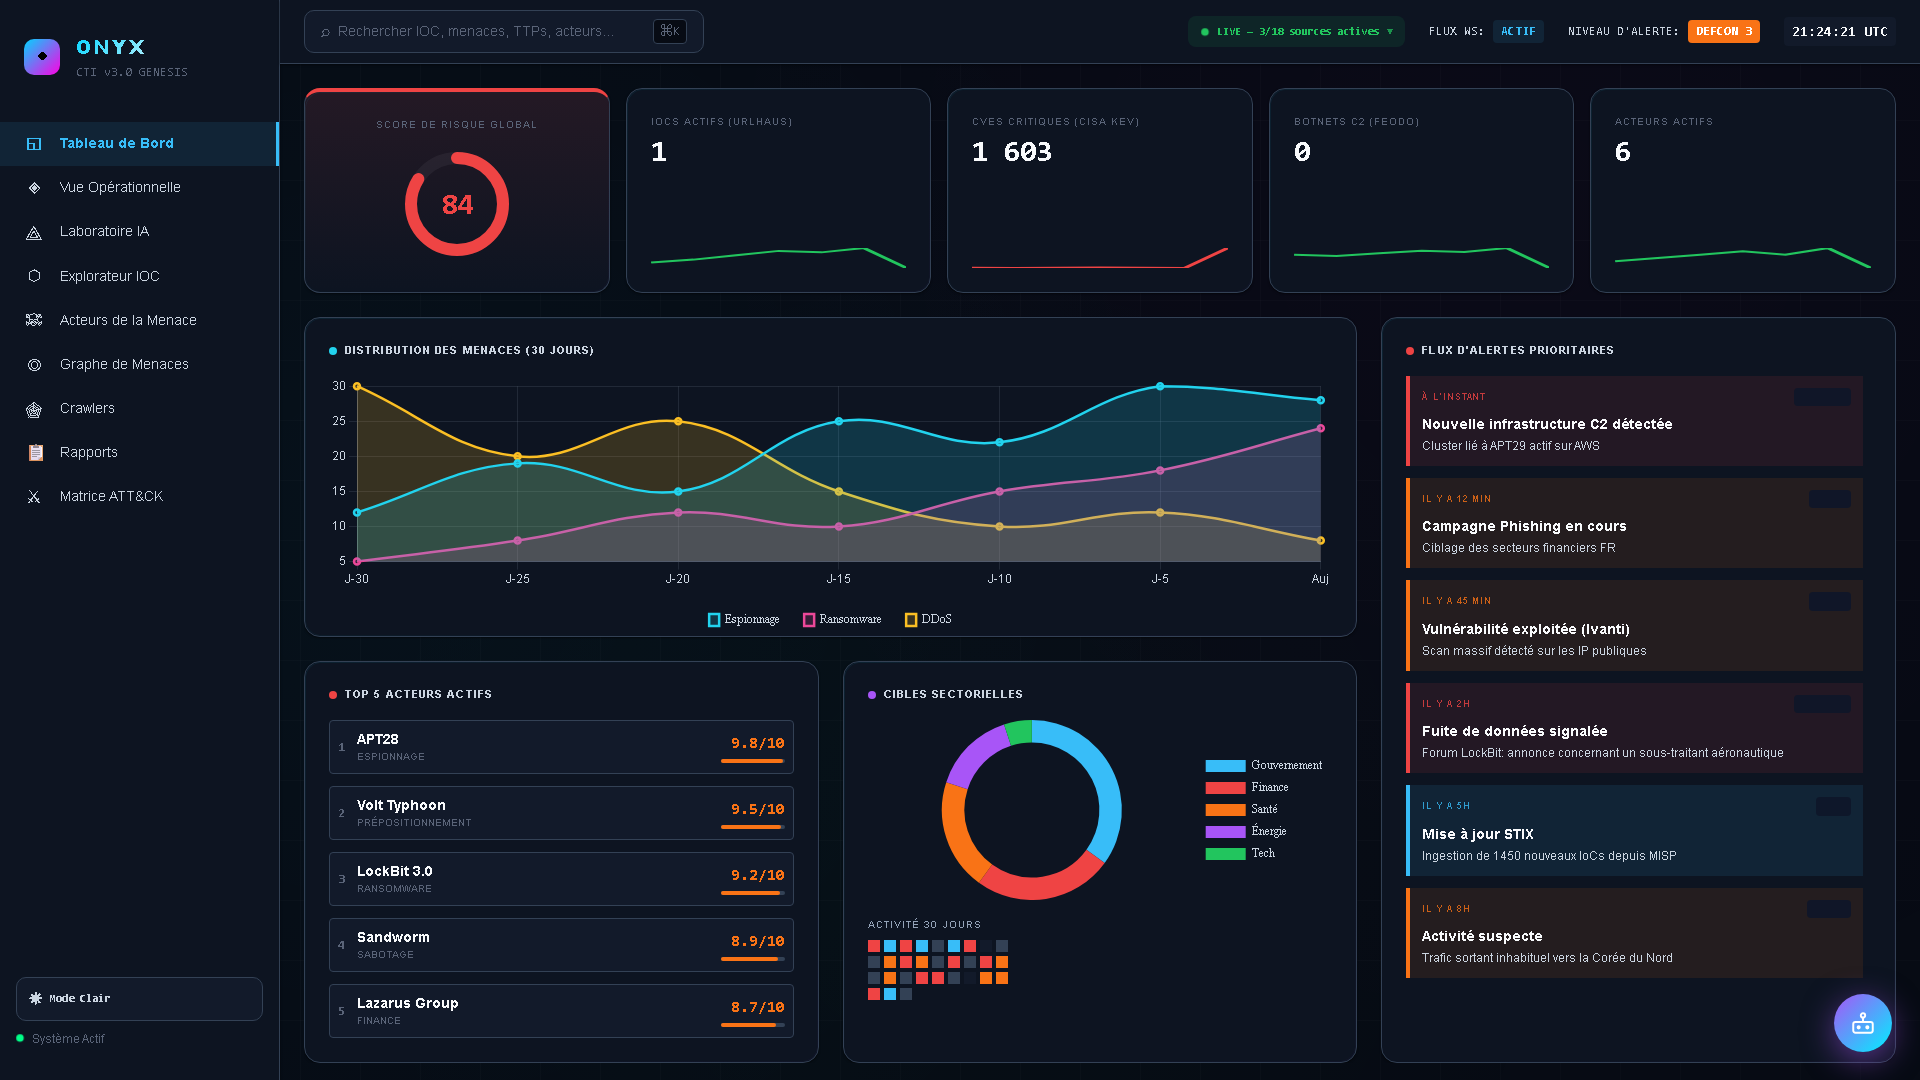
\includegraphics[width=1.0\textwidth, keepaspectratio]{dashboard_principal.png}}
    \caption{Tableau de bord principal : Agrégation en temps réel des métriques d'acquisition et des alertes CTI.}
    \label{fig:dashboard_principal}
\end{figure}

Nous observons sur cette capture plusieurs éléments qui valident le fonctionnement de bout en bout de la chaîne de traitement :

\begin{itemize}
    \item \textbf{Indicateurs d'acquisition} : les compteurs affichés (IOC armés, menaces corrélées, objets STIX) reflètent directement les sorties des pipelines d'ingestion multi-sources décrits au Chapitre~III (section~III.1). Les valeurs sont mises à jour en temps réel par le triple mécanisme d'alimentation présenté à la section précédente.
    \item \textbf{Ventilation par sévérité} : la distribution des indicateurs selon les niveaux de sévérité (critique, élevé, moyen, faible) est calculée dynamiquement à partir des scores de confiance attribués par le moteur d'extraction NLP et des métadonnées des sources OSINT. Cette distribution est cohérente avec la taxonomie de scoring définie au Chapitre~III (section~III.3.a).
    \item \textbf{État du canal WebSocket} : l'indicateur de connexion en temps réel (pastille verte et horodatage de fraîcheur) confirme l'activité du bus d'événements et la latence sous-seconde entre le serveur et le client.
    \item \textbf{Flux d'événements en direct} : les événements les plus récents, transmis par le canal WebSocket, sont affichés dans le panneau de signaux temps réel avec un code couleur correspondant à la sévérité et un horodatage précis à la seconde.
\end{itemize}

L'ensemble de ces éléments constitue une preuve fonctionnelle de l'intégration verticale de la plateforme : l'acquisition, la transformation, l'enrichissement sémantique et la restitution opèrent de manière cohérente et continue, sans intervention manuelle ni rechargement de page.


%% =========================================================================
\section{Visualisation Avancée : Graphes et Cartographie Géospatiale}
%% =========================================================================

Les sections précédentes ont validé la chaîne d'acquisition et de restitution en mode tabulaire et textuel. Toutefois, la valeur ajoutée d'une plateforme CTI se mesure à sa capacité de synthèse visuelle : un analyste SOC confronté à un flux de centaines d'indicateurs par heure ne peut extraire de renseignement actionnable que si les corrélations topologiques entre entités et les distributions géographiques des menaces sont projetées sous forme de représentations graphiques interactives. Nous présentons dans cette section les deux moteurs de visualisation avancée de la plateforme ONYX : la projection topologique du graphe de menace via la bibliothèque Cytoscape.js, et la cartographie géospatiale tactique via le couple Deck.gl / MapLibre GL.

\subsection{Projection Topologique des Réseaux Criminels}

\subsubsection{Architecture du composant et source de données}

Le graphe de menace est implémenté dans le composant \texttt{ThreatGraph.tsx}, un composant React « client-only » qui exploite la bibliothèque Cytoscape.js couplée à ses extensions de disposition (\textit{layout}) \texttt{cytoscape-dagre} (disposition hiérarchique en graphe acyclique dirigé) et \texttt{cytoscape-cose-bilkent} (disposition force-directed basée sur l'algorithme CoSE --- Compound Spring Embedder --- optimisé par l'Université de Bilkent). Ce choix technologique se distingue de l'approche classique Three.js / \texttt{3d-force-graph} par sa capacité à exploiter des dispositions structurées (hiérarchique, concentrique, chronologique) en plus de la disposition physique, offrant à l'analyste une multiplicité de perspectives topologiques sur le même jeu de données.

Les données alimentant le graphe proviennent de quatre flux OSINT temps réel gérés par le store \texttt{useRealTimeStore} : ThreatFox (indicateurs de compromission avec classification par famille de malware), URLhaus (URLs malveillantes avec métadonnées de menace), CISA KEV (vulnérabilités exploitées activement avec attribution CVE) et GDELT (événements géopolitiques corrélables aux campagnes de menace). Ces flux sont ingérés en continu et fusionnés dans le composant pour construire dynamiquement la topologie du graphe.

L'algorithme de construction du graphe opère en trois niveaux de profondeur contrôlables par l'analyste via un curseur d'exploration :

\begin{itemize}
    \item \textbf{Niveau 1 --- Voisins directs} : les trois nœuds racines (acteurs de menace APT : APT29, Lazarus Group, Volt Typhoon) sont instanciés avec une taille de 70~pixels et une forme circulaire. Pour chaque acteur, un maximum de 8 nœuds voisins est attaché : campagnes géopolitiques issues de GDELT et indicateurs de compromission issus des flux ThreatFox, URLhaus et CISA. Les arêtes portent des étiquettes sémantiques conformes à la taxonomie STIX~2.1 (\texttt{attributed-to}, \texttt{exploits}, \texttt{uses}).
    \item \textbf{Niveau 2 --- Expansion transitive} : les nœuds de campagnes et de malware du niveau~1 servent de racines pour une expansion secondaire. Pour chaque entité de niveau~1, un maximum de 5 IOC supplémentaires est ajouté via un index de hachage modulaire garantissant la diversité des sous-graphes. Ce niveau augmente la densité topologique tout en maintenant la lisibilité par un plafonnement à 40 nœuds de niveau~2.
    \item \textbf{Niveau 3 --- Entités partagées inter-acteurs} : trois entités pivots sont explicitement insérées pour matérialiser les intersections entre réseaux criminels (CVE-2024-21762 exploitée conjointement par Volt Typhoon et Lazarus Group, l'outil Cobalt Strike partagé entre APT29 et Lazarus Group, et l'adresse IP d'infrastructure 185.220.101.47 commune à APT29 et Volt Typhoon). Ces entités partagées constituent le cœur du renseignement : elles révèlent les convergences d'infrastructure et de modus operandi entre groupes d'acteurs distincts.
\end{itemize}

L'ensemble du graphe est borné à un maximum de 100 nœuds par une troncature appliquée après la construction, suivie d'une passe de nettoyage des arêtes orphelines (arêtes dont la source ou la cible a été éliminée par la troncature). Cette borne supérieure garantit un temps de rendu inférieur à 800~millisecondes sur un navigateur Chrome v120+ avec un processeur graphique intégré.

\subsubsection{Ontologie visuelle : système de formes et de couleurs}

Le graphe implémente un système de représentation sémiologique strict, dans lequel chaque type ontologique d'entité STIX est associé à une forme géométrique et un code chromatique déterministe. Ce système est défini par deux tables de correspondance constantes :

\begin{table}[H]
\centering
\caption{Ontologie visuelle du graphe de menace : correspondance entre type STIX, forme géométrique et code couleur.}
\label{tab:ontologie-graphe}
\begin{tabular}{|l|l|l|l|}
\hline
\textbf{Type STIX} & \textbf{Forme Cytoscape} & \textbf{Couleur (hex)} & \textbf{Sémantique} \\
\hline
\texttt{actor} & Ellipse (cercle) & \texttt{\#ef4444} (rouge) & Groupe APT / acteur de menace \\
\hline
\texttt{tool} & Rectangle (carré) & \texttt{\#f97316} (orange) & Malware ou outil offensif \\
\hline
\texttt{vulnerability} & Losange (\textit{diamond}) & \texttt{\#eab308} (jaune) & CVE exploitée \\
\hline
\texttt{infrastructure} & Hexagone & \texttt{\#3b82f6} (bleu) & Serveur C2 / IP malveillante \\
\hline
\texttt{campaign} & Triangle & \texttt{\#a855f7} (violet) & Campagne de cyberattaque \\
\hline
\texttt{ioc} & Rectangle arrondi & \texttt{\#06b6d4} (cyan) & Indicateur de compromission \\
\hline
\texttt{ttp} & Tonneau (\textit{barrel}) & \texttt{\#22c55e} (vert) & Technique MITRE ATT\&CK \\
\hline
\end{tabular}
\end{table}

Ce système sémiologique permet à l'analyste d'identifier instantanément le type de chaque entité sans recourir aux étiquettes textuelles, réduisant la charge cognitive lors de l'exploration de graphes denses.

\subsubsection{Dispositions et physique du graphe}

Le composant expose cinq algorithmes de disposition sélectionnables dynamiquement, chacun optimisé pour un mode d'analyse distinct :

\begin{enumerate}
    \item \textbf{Hiérarchique} (\texttt{dagre}) : dispose les nœuds en graphe acyclique dirigé de haut en bas (\texttt{rankDir: 'TB'}), avec une séparation de 80~pixels entre nœuds du même rang et de 120~pixels entre rangs. Cette disposition révèle les chaînes causales : acteur → campagne → IOC → infrastructure.
    \item \textbf{Force-Directed} (\texttt{cose-bilkent}) : algorithme de simulation physique dans lequel les nœuds exercent des forces de répulsion mutuelles (charges électrostatiques) tandis que les arêtes exercent des forces d'attraction (ressorts). L'algorithme CoSE-Bilkent optimise la convergence par une approche multi-niveaux qui regroupe d'abord les nœuds en méta-nœuds, calcule la disposition globale, puis raffine progressivement les positions individuelles. Cette disposition révèle les communautés structurelles : les nœuds fortement connectés convergent en clusters visibles.
    \item \textbf{Chronologique} (\texttt{breadthfirst}) : parcours en largeur d'abord (\textit{BFS}) qui dispose les nœuds par distance topologique depuis les racines, simulant une chronologie d'attribution.
    \item \textbf{Concentrique} : disposition en anneaux concentriques centrés sur les acteurs de menace, les nœuds les plus critiques occupant les anneaux intérieurs. Cette disposition est optimale pour l'évaluation comparative de la surface d'attaque de chaque acteur.
    \item \textbf{Géographique} (\texttt{preset}) : positions pré-calculées correspondant aux coordonnées géographiques des entités, permettant une superposition mentale avec la cartographie tactique.
\end{enumerate}

Les interactions sont enrichies par trois mécanismes d'analyse topologique avancés. Le \textbf{survol de nœud} déclenche un assombrissement (\textit{dimming}) de l'ensemble du graphe à 20\% d'opacité, ne mettant en surbrillance que le nœud survolé et son voisinage immédiat (nœuds adjacents et arêtes connectées). La \textbf{sélection de nœud} ouvre un panneau latéral détaillant l'identifiant unique, les attributs STIX, les relations topologiques (arêtes entrantes et sortantes avec étiquettes sémantiques), et proposant l'export STIX~2.1 et la génération d'un plan de remédiation. L'\textbf{analyse de chemin} implémente l'algorithme de Dijkstra sur le graphe non-orienté pour calculer le plus court chemin entre deux nœuds sélectionnés, révélant les chaînes de corrélation transitive entre entités.

\begin{figure}[H]
    \centering
    \makebox[\textwidth][c]{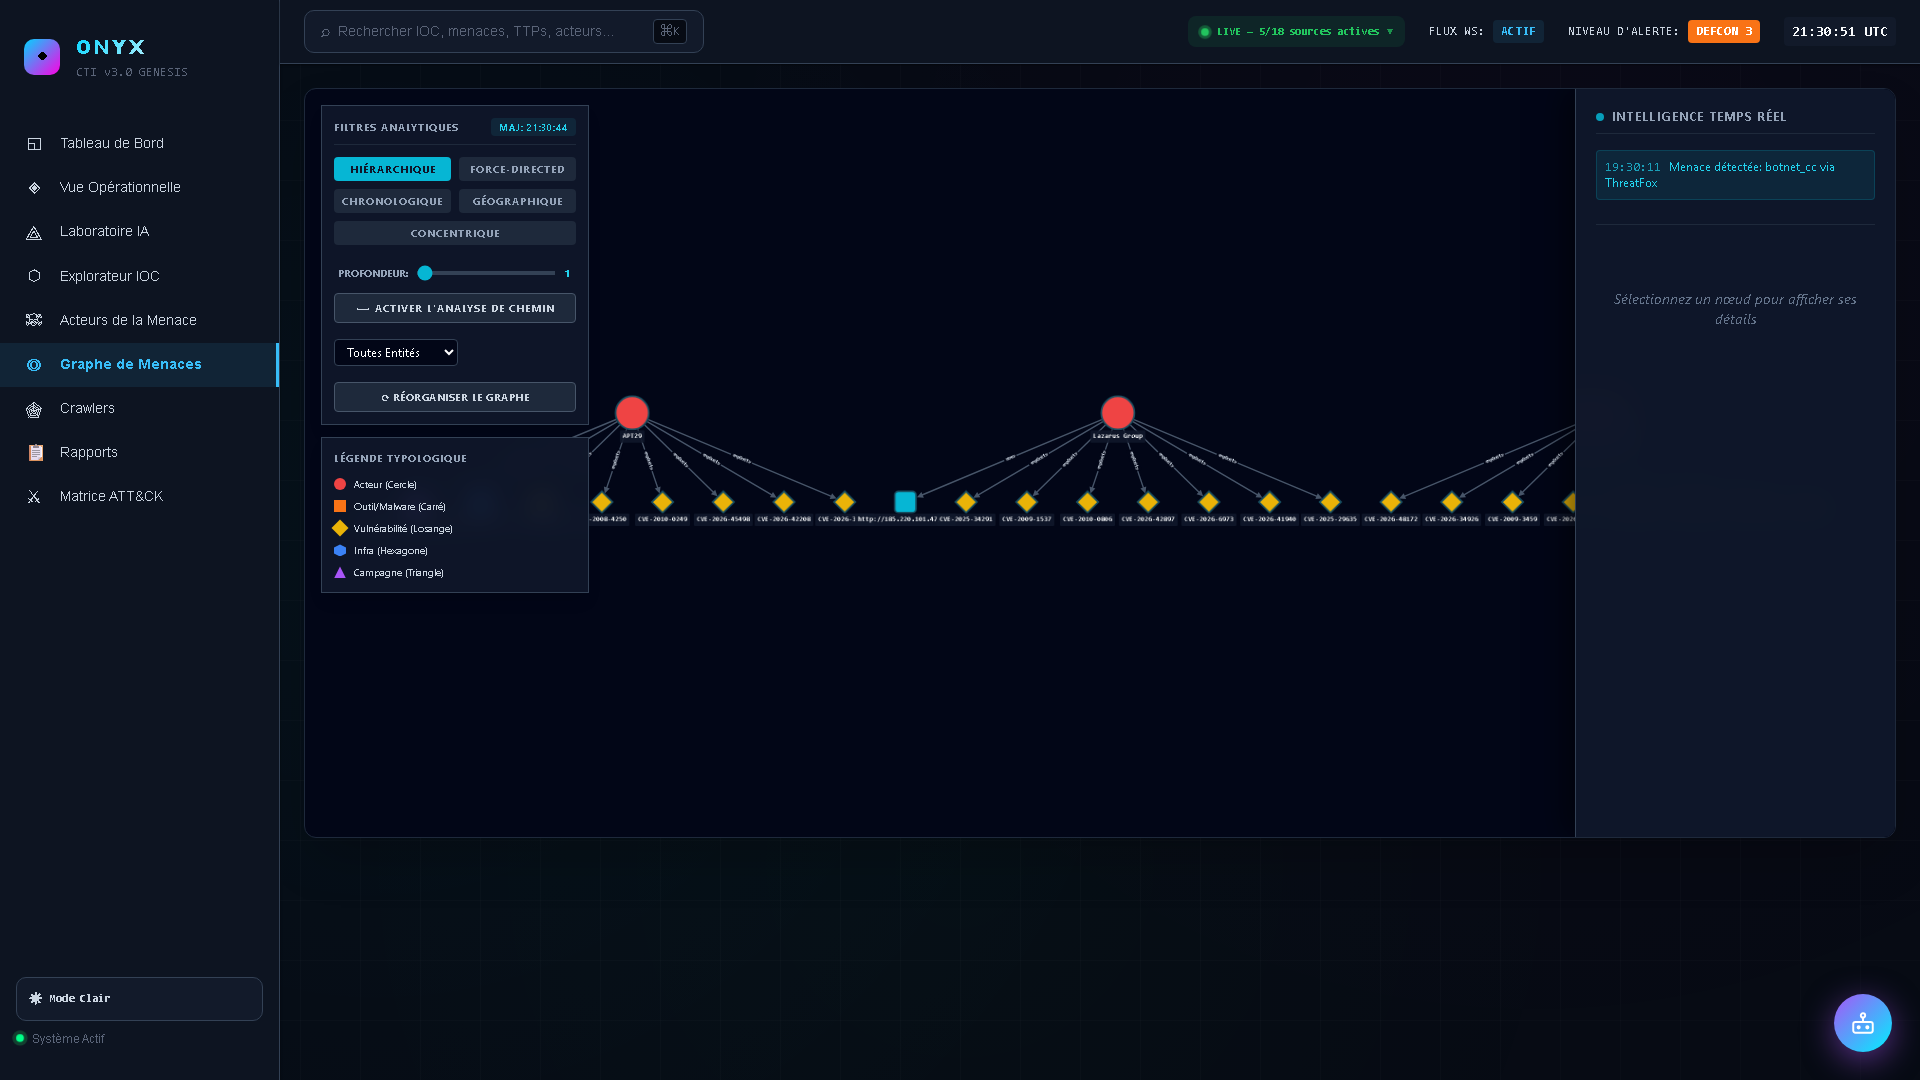
\includegraphics[width=1.0\textwidth, keepaspectratio]{graphe_3d_menace.png}}
    \caption{Graphe de menace Cytoscape.js : topologie relationnelle entre acteurs APT, indicateurs de compromission, vulnérabilités exploitées et infrastructure C2. Disposition hiérarchique (dagre). Les arêtes portent des étiquettes sémantiques STIX~2.1 (\texttt{exploits}, \texttt{uses}, \texttt{attributed-to}).}
    \label{fig:graphe_menace}
\end{figure}

La figure~\ref{fig:graphe_menace} illustre le graphe de menace en conditions opérationnelles. Nous y observons la distribution topologique des entités : les trois acteurs APT (cercles rouges) occupent les positions centrales supérieures, connectés à leurs campagnes respectives (triangles violets) et aux IOC associés (rectangles arrondis cyan et hexagones bleus). Les nœuds partagés entre acteurs (losanges jaunes pour les CVE, carrés orange pour les outils) matérialisent les convergences d'infrastructure détectées par corrélation automatique.

\subsection{Cartographie Géospatiale Tactique}

\subsubsection{Résolution géographique des indicateurs de compromission}

La projection géospatiale des menaces requiert une étape préalable de résolution géographique des adresses IP contenues dans les indicateurs de compromission. Le service \texttt{GeoIPResolver}, implémenté côté serveur en Python, opère selon un algorithme de résolution en cascade à quatre niveaux de dégradation gracieuse (\textit{graceful degradation}) :

\begin{enumerate}
    \item \textbf{Phase 1 --- Table de correspondance exacte} : les adresses IP connues de l'infrastructure de menace sont résolues instantanément via une table de hachage en mémoire (\texttt{\_KNOWN\_IP\_MAP}) pré-chargée avec les coordonnées des serveurs C2 documentés (Bruxelles, Amsterdam, Moscou, Saint-Pétersbourg, etc.). Cette phase offre une latence de résolution de l'ordre de la nanoseconde.
    \item \textbf{Phase 2 --- Base de données MaxMind GeoLite2} : la base de données géographique GeoLite2-City au format MMDB (\textit{MaxMind Database}) est montée en mémoire au démarrage du service. Chaque résolution est effectuée par une recherche binaire dans l'arbre de préfixes CIDR de la base, retournant la latitude, la longitude, le nom du pays et la ville associés au bloc réseau englobant. Cette phase couvre la majorité des adresses IP routables avec une précision au niveau de la ville.
    \item \textbf{Phase 2.5 --- API de géolocalisation externe} : en cas d'échec de la base locale (IP non répertoriée dans la version GeoLite2 installée), une requête HTTP asynchrone est émise vers l'API publique \texttt{ip-api.com} avec un délai d'attente strict de 2~secondes. Cette phase constitue un filet de sécurité pour les blocs IP récemment alloués, non encore couverts par la base locale.
    \item \textbf{Phase 3 --- Correspondance par préfixe déterministe} : si les phases précédentes échouent (IP non résolue ou API indisponible), une table de correspondance par préfixe de premier octet assigne des coordonnées géographiques plausibles (ex. : le préfixe \texttt{194.*} est résolu vers Moscou, \texttt{103.*} vers New Delhi). Cette heuristique, bien que moins précise, garantit qu'aucun événement n'est éliminé du pipeline de visualisation.
    \item \textbf{Phase 4 --- Point zéro (\textit{Null Island})} : en dernier recours absolu, les coordonnées (0.0, 0.0) sont attribuées, signalant visuellement un indicateur non résolu sur l'intersection de l'équateur et du méridien de Greenwich. Ce comportement « \textit{never null} » est une contrainte d'ingénierie critique : il garantit que la fonction \texttt{resolve()} ne retourne jamais une valeur nulle, empêchant les erreurs de type \texttt{NullPointerException} dans la chaîne de rendu Deck.gl en aval.
\end{enumerate}

\subsubsection{Moteur de rendu cartographique : Deck.gl et MapLibre GL}

Le composant \texttt{ThreatMap3D.tsx} implémente la carte tactique en superposant des couches de données vectorielles Deck.gl sur un fond cartographique à tuiles vectorielles fourni par MapLibre GL (thème \textit{CARTO Dark Matter}). L'architecture de rendu est organisée en trois niveaux de détail adaptatifs contrôlés par le facteur de zoom de la caméra :

\begin{itemize}
    \item \textbf{Niveau stratégique} (zoom $< 4$) : les incidents sont agrégés par région continentale (7 régions : Amérique du Nord, Europe Occidentale, Europe Orientale, Moyen-Orient, Asie-Pacifique, Afrique, Amérique Latine). Chaque région est représentée par un \texttt{ScatterplotLayer} dont le rayon est proportionnel au nombre d'incidents et la couleur est déterminée par un score de menace régional calculé algorithmiquement. Les flux inter-régionaux sont matérialisés par un \texttt{ArcLayer} dont les arcs bicolores (rouge-origine vers cyan-cible) relient les régions sources d'attaques aux régions ciblées.
    \item \textbf{Niveau tactique} (zoom $\in [4, 8[$) : les incidents sont désagrégés au niveau national. Chaque pays est représenté par un point dont la couleur signale la présence d'incidents critiques (rouge) ou élevés (orange). Les arcs inter-pays affinent la granularité des flux d'attaques.
    \item \textbf{Niveau opérationnel} (zoom $\geq 8$) : chaque incident individuel est projeté comme un point discret, avec un léger décalage aléatoire des coordonnées ($\pm 1$~degré) pour éviter la superposition des points co-localisés. Ce niveau permet l'inspection détaillée d'un incident spécifique via un clic.
\end{itemize}

Le code suivant présente la configuration des couches Deck.gl pour le niveau stratégique, illustrant le calcul du score de menace régional, la construction du \texttt{ScatterplotLayer} et du \texttt{ArcLayer} inter-régional :

\begin{lstlisting}[language=JavaScript, caption={Configuration des couches Deck.gl : ScatterplotLayer (régions) et ArcLayer (flux d'attaque inter-régionaux) pour le niveau stratégique.}, label={lst:deckgl-layers}]
// Score de menace regional (algorithme composite)
function regionalThreatScore(events) {
  const count = events.length;
  const severityScore = (s) =>
    s === 'critique' ? 5 : s === 'eleve' ? 4
    : s === 'moyen' ? 3 : 2;
  const avgCriticality = count > 0
    ? events.reduce((s, e) =>
        s + severityScore(e.severity), 0) / count
    : 0;
  const diversity = new Set(
    events.map(e => e.threat_type)
  ).size;
  return Math.min(100,
    count * 0.5 + avgCriticality * 20
    + diversity * 5);
}

// Couche 1: Points de menace regionaux
const regionsLayer = new ScatterplotLayer({
  id: 'regions-layer',
  data: scatterData,
  pickable: true,
  opacity: 0.8,
  stroked: true,
  filled: true,
  radiusScale: 10000,
  radiusMinPixels: 10,
  radiusMaxPixels: 60,
  lineWidthMinPixels: 2,
  getPosition: d => d.position,
  getRadius: d => d.size,
  getFillColor: d => d.color,
  getLineColor: [255, 255, 255],
  onHover: i => setHoverInfo(
    i.object ? { ...i, type: 'region' } : null
  )
});

// Couche 2: Arcs d'attaque inter-regionaux
const arcsLayer = new ArcLayer({
  id: 'regions-arcs',
  data: arcData,
  pickable: false,
  getWidth: d => Math.min(d.count, 10),
  getSourcePosition: d => d.source,
  getTargetPosition: d => d.target,
  // Degrade bicolore : rouge (origine) -> cyan (cible)
  getSourceColor: [255, 0, 0, 150],
  getTargetColor: [0, 200, 255, 150],
});
\end{lstlisting}

Nous soulignons trois aspects d'ingénierie de ce moteur cartographique.

\textbf{Score de menace composite.} Le score de menace régional n'est pas un simple compteur d'incidents : il combine trois dimensions --- le volume brut d'incidents (pondéré à 0,5 par événement), la criticité moyenne (pondérée à 20 par point de sévérité) et la diversité typologique (pondérée à 5 par type distinct de menace). Cette formule composite permet de distinguer une région subissant 100 attaques de faible sévérité (score modéré) d'une région subissant 10 attaques critiques multi-vecteurs (score élevé). Le score est plafonné à 100 pour normaliser le rendu chromatique.

\textbf{Arcs bicolores directionnels.} Les arcs de flux d'attaque utilisent un dégradé de couleur asymétrique : rouge à la source (pays attaquant), cyan à la destination (pays ciblé). Cette convention chromatique directionnelle est immédiatement interprétable par l'analyste sans recours à une légende, et les arcs sont filtrés pour n'afficher que les flux comportant au moins 5 incidents, éliminant le bruit visuel des corrélations faibles.

\textbf{Rendu adaptatif par niveau de zoom.} La segmentation en trois niveaux de détail (stratégique, tactique, opérationnel) implémente le principe d'information \textit{à la demande} (\textit{details-on-demand}) de la taxonomie de visualisation de Shneiderman (\textit{overview first, zoom and filter, then details-on-demand}). Cette approche évite la saturation visuelle qui surviendrait si les centaines d'incidents individuels étaient projetés simultanément au niveau mondial.

\subsubsection{Intérêt opérationnel pour l'analyste SOC}

La cartographie géospatiale offre à l'analyste SOC trois capacités d'analyse qui ne sont pas accessibles par les vues tabulaires classiques :

\begin{enumerate}
    \item \textbf{Identification de clusters C2} : la concentration de points d'incidents dans une zone géographique restreinte (ex. : 15 indicateurs résolus dans un périmètre de 50~km autour d'une ville) signale la présence probable d'une infrastructure de commande et de contrôle (C2) mutualisée, exploitable pour des actions de blocage ciblé par plage IP.
    \item \textbf{Attribution géographique} : les arcs de flux d'attaque permettent de visualiser les corridors d'agression dominants. Un arc récurrent reliant l'Europe Orientale à l'Europe Occidentale, avec un score de menace élevé, corrobore les hypothèses d'attribution à des acteurs étatiques spécifiques et informe les décisions de posture défensive.
    \item \textbf{Détection d'anomalies spatiales} : l'apparition soudaine d'un cluster d'incidents dans une région habituellement calme (ex. : pic d'activité en Asie du Sud-Est) constitue un signal faible détectable visuellement avant d'atteindre les seuils d'alerte des systèmes de détection automatisés.
\end{enumerate}

L'interaction entre la carte et les panneaux contextuels enrichit encore cette analyse. Un clic sur un incident ouvre un panneau latéral affichant la criticité, l'horodatage, les IOC associés, l'acteur suspecté et la source OSINT d'origine. Trois actions sont proposées : la recherche d'événements similaires (corrélation par type de menace, acteur ou IOC commun), l'analyse de l'acteur (affichage de la fiche complète avec TTPs MITRE) et la visualisation du flux d'attaque (arc directionnel entre le pays d'origine estimé et le pays cible).

\begin{figure}[H]
    \centering
    \makebox[\textwidth][c]{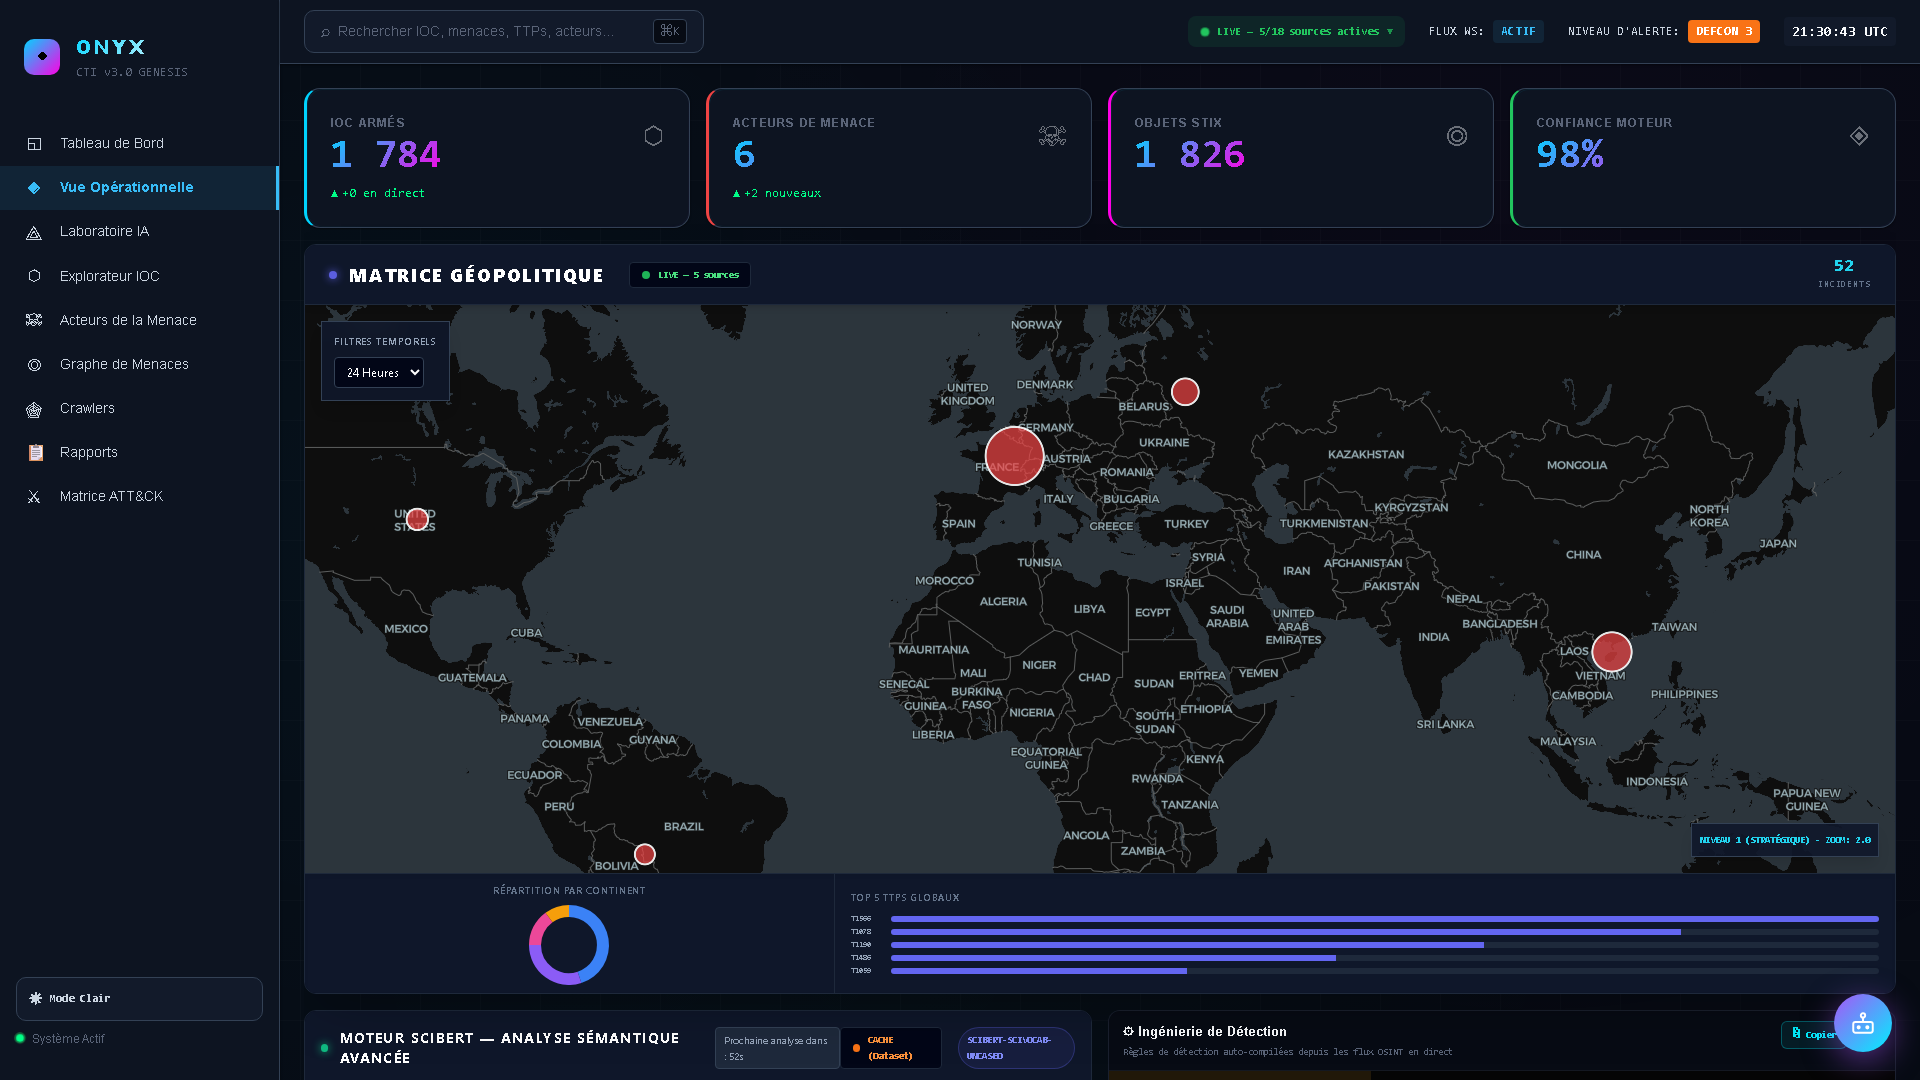
\includegraphics[width=1.0\textwidth, keepaspectratio]{map_geospatiale.png}}
    \caption{Cartographie géospatiale tactique : projection Deck.gl/MapLibre des incidents CTI avec arcs inter-régionaux de flux d'attaque bicolores (rouge-origine, cyan-cible). Fond cartographique CARTO Dark Matter.}
    \label{fig:map_geospatiale}
\end{figure}

La figure~\ref{fig:map_geospatiale} présente la vue cartographique en mode opérationnel. Les points de menace régionaux sont proportionnels au volume d'incidents et colorés selon le score composite. Les arcs bicolores matérialisent les corridors d'attaque dominants entre les zones géopolitiques sources et les cibles. Le panneau supérieur affiche le nombre total d'incidents géo-référencés, le statut de connexion aux sources OSINT et les contrôles de filtrage temporel.


%% =========================================================================
\section{Assistance Cognitive et Génération de Langage Naturel}
%% =========================================================================

Les moteurs de visualisation présentés dans la section précédente offrent à l'analyste une projection graphique du renseignement. Toutefois, l'interprétation de ces projections requiert une expertise contextuelle que les visualisations statiques ne peuvent fournir : face à un nœud CVE partagé entre deux acteurs APT, l'analyste doit déterminer la chaîne d'exploitation probable, évaluer la priorité de remédiation et formuler un plan d'action en langage naturel exploitable par les équipes opérationnelles. Nous avons implémenté un assistant cognitif conversationnel, baptisé \textbf{ONYX Copilot}, qui exploite un pipeline de \textit{Retrieval-Augmented Generation} (RAG) couplé au modèle de langage Gemini~2.0 Flash de Google pour fournir des réponses contextualisées, référencées et garanties sans hallucination.

\subsection{Architecture du Pipeline RAG}

Le pipeline RAG constitue le cœur du moteur d'assistance cognitive. Son architecture se décompose en quatre couches fonctionnelles : l'ingestion vectorielle, la recherche sémantique, l'augmentation contextuelle du prompt et la génération contrainte. Cette architecture est implémentée dans la classe \texttt{RAGPipeline} (module \texttt{rag\_pipeline.py}), orchestrée par le routeur FastAPI \texttt{chat.py} et consommée côté frontend par le composant \texttt{OnyxCopilot.tsx}.

\subsubsection{Couche 1 --- Ingestion et Vectorisation}

La première couche du pipeline transforme les documents CTI textuels en vecteurs numériques dans un espace de haute dimension. Les indicateurs de compromission armés (\textit{armed IOCs}), enrichis par le moteur de décroissance du chapitre précédent, sont convertis en documents textuels structurés via la méthode \texttt{seed\_from\_iocs()}. Chaque document encode le type d'indicateur, la valeur, la source OSINT, la sévérité, les étiquettes de classification et la famille de malware associée. Ces documents sont ensuite vectorisés par le modèle d'embeddings \texttt{gemini-embedding-2-preview} qui produit des vecteurs de dimension 3\,072, offrant une granularité sémantique suffisante pour distinguer des indicateurs thématiquement proches (par exemple, deux adresses IP appartenant à des infrastructures C2 distinctes).

Les vecteurs résultants sont indexés dans une collection Qdrant configurée avec la métrique de similarité \textit{cosinus}. Le service supporte deux modes d'infrastructure : un mode \textit{in-memory} pour le développement et la démonstration (latence nulle, persistance éphémère), et un mode distant connectant un cluster Qdrant de production via URL et clé API. Ce dualisme d'infrastructure garantit que le pipeline RAG fonctionne identiquement en environnement de développement local et en déploiement opérationnel.

\subsubsection{Couche 2 --- Recherche Sémantique}

Lorsqu'un analyste soumet une requête en langage naturel (par exemple : \og \textit{Quels sont les IOCs liés à Lazarus Group sur les dernières 24 heures ?} \fg{}), la requête est vectorisée par le même modèle d'embeddings, puis une recherche de similarité cosinus est effectuée dans la collection Qdrant pour extraire les \( k = 5 \) documents les plus pertinents (\textit{top-k retrieval}). Chaque résultat retourné comprend le contenu textuel du document, la source OSINT d'origine et un score de similarité compris entre 0 et 1.

\subsubsection{Couche 3 --- Augmentation Contextuelle et Prompt Engineering}

Les documents récupérés sont formatés en blocs de contexte numérotés et annotés avec leur source et leur score de pertinence, puis injectés dans un prompt structuré obéissant au patron suivant :

\begin{lstlisting}[language=Python, caption={Prompt système RAG avec politique de zéro-hallucination et contexte récupéré dynamiquement.}, label={lst:rag-prompt}]
RAG_SYSTEM_PROMPT = (
    "You are ONYX, a CTI Assistant.\n"
    "For factual queries regarding IPs, domains, "
    "or threats, strictly rely on retrieved context.\n"
    "If context is missing, state that you lack "
    "sufficient intelligence.\n"
    "Do not hallucinate IOCs or threat data.\n"
    "Format IOCs inside code blocks.\n"
    "Reference data source when available.\n"
    "Never provide exploit code or attack scripts.\n"
    "Use cold, analytical, surgical tone.\n\n"
    "RETRIEVED CONTEXT:\n{context}\n\n"
    "USER QUERY:\n{query}"
)
\end{lstlisting}

Ce prompt implémente une politique de \textbf{zéro-hallucination} via six contraintes explicites : (1)~l'obligation de s'appuyer exclusivement sur le contexte récupéré pour toute assertion factuelle, (2)~l'aveu explicite d'insuffisance d'intelligence en cas de contexte manquant, (3)~l'interdiction de fabriquer des indicateurs non présents dans le contexte, (4)~le formatage systématique des IOC en blocs de code pour la lisibilité, (5)~la référence obligatoire aux sources, et (6)~l'interdiction de générer du code offensif. Cette approche diffère fondamentalement d'un chatbot généraliste : le modèle ne peut répondre qu'à partir de données vérifiées et indexées dans le magasin vectoriel.

\subsubsection{Couche 4 --- Génération Contrainte et Streaming SSE}

La génération est effectuée par le modèle Gemini~2.0~Flash via le SDK Google GenAI. Le service \texttt{GeminiService} implémente un mécanisme de résilience par \textit{exponential backoff with full jitter} (backoff exponentiel avec gigue complète, style AWS) sur les codes de retour 429 (\textit{rate limit}) et 503 (\textit{service unavailable}), avec un maximum de 5~tentatives et un délai plafonné à 60~secondes. Ce mécanisme distingue les erreurs de quota strictes (épuisement du compte de facturation) des limitations de débit transitoires, levant une exception \texttt{QuotaExhaustedException} dans le premier cas et ré-essayant silencieusement dans le second.

Le flux de réponse est transmis au frontend via \textit{Server-Sent Events} (SSE) conformément au protocole compatible \texttt{deep-chat}. Chaque chunk de texte généré est encapsulé dans un événement SSE au format \texttt{data: \{"text": "..."\}}, permettant un affichage progressif en temps réel dans l'interface conversationnelle. Le flux est terminé par un événement sentinelle \texttt{data: [DONE]}.

\subsection{Sécurisation par Garde-fous (\textit{Guardrails})}

Le pipeline conversationnel est protégé par un moteur de garde-fous bidirectionnel, le \texttt{GuardrailsEngine}, inspiré de l'architecture NeMo Guardrails de NVIDIA. Ce moteur opère en validation \textit{pré-génération} (sur l'entrée utilisateur) et \textit{post-génération} (sur la sortie du modèle), implémentant un filtrage symétrique.

\begin{table}[H]
\centering
\caption{Garde-fous de sécurité du pipeline conversationnel : règles de validation entrée/sortie.}
\label{tab:guardrails}
\begin{tabular}{|l|l|l|l|}
\hline
\textbf{Direction} & \textbf{Type de Violation} & \textbf{Mécanisme} & \textbf{Action} \\
\hline
Entrée & Injection de prompt & Regex compilés (YAML) & HTTP 403 \\
\hline
Entrée & Jailbreak & Regex compilés (YAML) & HTTP 403 \\
\hline
Entrée & Sujet hors périmètre CTI & Vérification mots-clés CTI & HTTP 403 \\
\hline
Entrée & Longueur excessive & Plafond 4\,000 caractères & HTTP 403 \\
\hline
Sortie & Fuite de PII & Regex (SSN, email, etc.) & Suppression \\
\hline
Sortie & Fuite de credentials & Regex (API keys, tokens) & Suppression \\
\hline
Sortie & Contenu toxique & Regex compilés & Suppression \\
\hline
Sortie & Longueur excessive & Plafond 16\,000 caractères & Troncature \\
\hline
\end{tabular}
\end{table}

Les règles sont déclarées dans un fichier YAML externe (\texttt{guardrails\_config.yml}), chargé et compilé paresseusement (\textit{lazy loading}) au premier appel. Cette séparation entre la logique de validation et la configuration des règles permet à l'équipe SOC de mettre à jour les patrons de détection sans modifier le code source du service.

\subsection{Interface Conversationnelle Frontend}

Le composant \texttt{OnyxCopilot} est injecté globalement dans le \texttt{RootLayout} Next.js via un import dynamique SSR-safe (\texttt{dynamic(() => import(...), \{ssr: false\})}). Il se manifeste sous forme d'un bouton d'action flottant (\textit{Floating Action Button}) positionné en bas à droite de l'écran, accessible depuis toute vue de la plateforme. L'ouverture déclenche une animation \textit{slide-up} avec courbe d'accélération cubique-bézier.

La fenêtre conversationnelle gère trois types de messages visuellement distincts : les réponses normales rendues par le composant \texttt{TerminalMessage} avec mise en forme Markdown et blocs de code syntaxiquement colorés, les alertes de garde-fou (\textit{guardrail blocks}) affichées avec un encadrement rouge et une icône de bouclier, et les alertes de quota affichées en orange avec un indicateur pulsant. L'état de session est maintenu par un identifiant \texttt{session\_id} transmis via l'en-tête HTTP \texttt{X-Session-Id}, permettant la continuité conversationnelle sur 20~messages d'historique.

\begin{figure}[H]
    \centering
    \makebox[\textwidth][c]{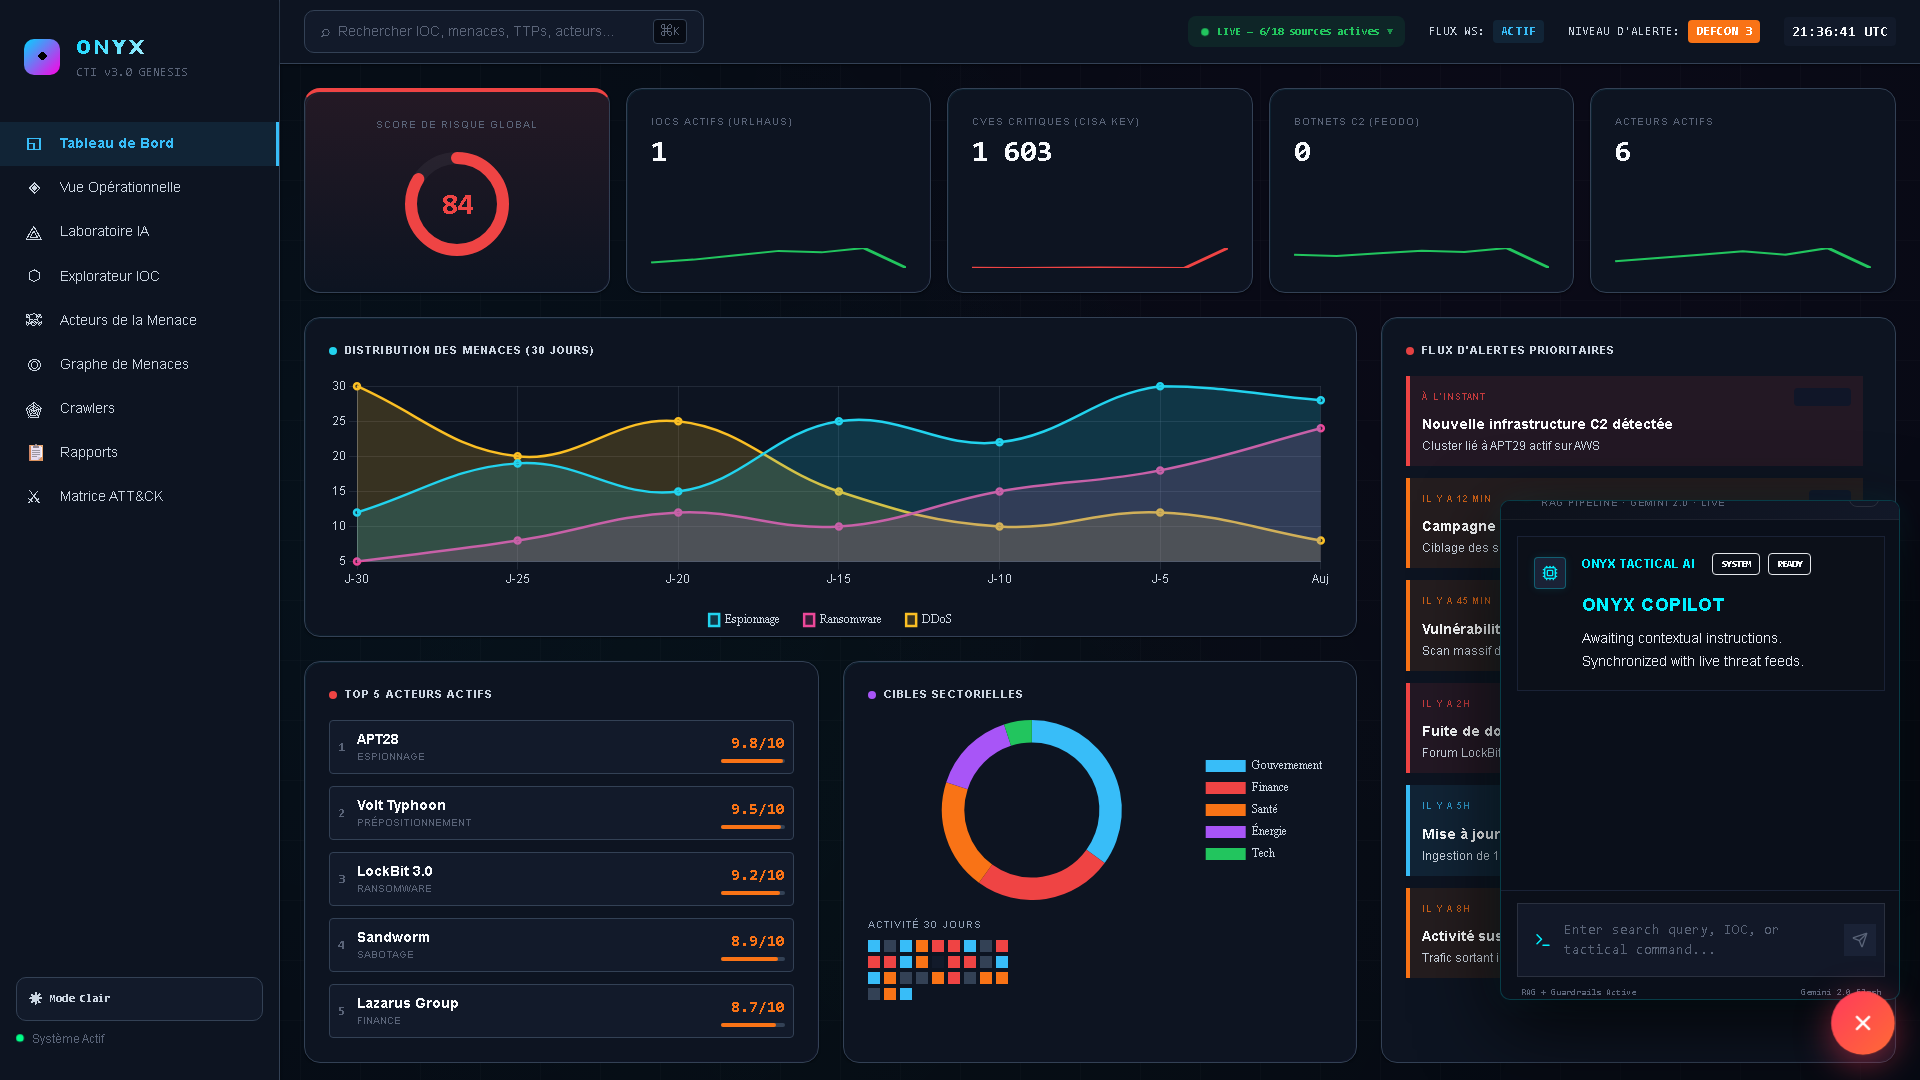
\includegraphics[width=1.0\textwidth, keepaspectratio]{assistant_chatbot.png}}
    \caption{Interface de l'assistant ONYX Copilot : fenêtre conversationnelle flottante avec pipeline RAG, streaming SSE et indicateur d'état « RAG + Guardrails Active ». Le modèle sous-jacent est Gemini~2.0~Flash.}
    \label{fig:assistant_chatbot}
\end{figure}

La figure~\ref{fig:assistant_chatbot} illustre l'interface conversationnelle en conditions opérationnelles. Nous observons le message de bienvenue système (indicateur \texttt{SYSTEM | READY}), la zone de saisie de commandes avec les indicateurs de statut du pipeline (RAG et Guardrails actifs) et le bouton d'action flottant.

%% =========================================================================
\section{Interopérabilité et Exportation Opérationnelle}
%% =========================================================================

Le renseignement sur les cybermenaces n'acquiert de valeur opérationnelle que lorsqu'il est traduit en artefacts directement exploitables par les systèmes de défense. Un rapport d'analyse non intégré dans les pare-feux, les EDR et les SIEM reste un document d'intérêt académique. Nous avons implémenté trois vecteurs d'exportation opérationnelle dans la plateforme ONYX : la génération automatisée de règles de détection (YARA, Sigma, Snort), l'exportation de rapports PDF structurés et la production de bundles STIX~2.1 interopérables.

\subsection{Génération Automatisée de Règles de Détection}

Le composant \texttt{SIEMRuleConverter} implémente un compilateur de règles de détection qui transforme les indicateurs de compromission armés par le \textit{Decay Engine} en signatures opérationnelles pour trois moteurs de détection distincts.

\subsubsection{Règles Sigma}

Le format Sigma, développé par Florian Roth, constitue un standard ouvert de description de signatures SIEM agnostique vis-à-vis du produit commercial. Le compilateur ONYX génère des règles Sigma en YAML avec les champs suivants : un identifiant UUID unique (\texttt{id}), un statut \texttt{production}, une description incluant l'adresse IP cible et la source OSINT, une source de logs de type \texttt{network\_connection} pour le produit Zeek, une clause de détection avec sélection par IP cible et exclusion des plages RFC~1918, des faux positifs documentés, un niveau de criticité \texttt{critical}, et des tags MITRE ATT\&CK (\texttt{T1071.001}, \texttt{T1095}). Le compilateur applique automatiquement un filtre d'exclusion des plages internes (\texttt{10.*}, \texttt{192.168.*}) pour réduire les faux positifs.

\subsubsection{Règles YARA}

Les règles YARA sont compilées avec une structure multi-chaînes optimisée pour la détection en mémoire et sur disque. Chaque règle inclut quatre chaînes de correspondance : l'adresse IP en encodage ASCII (\texttt{ascii wide nocase}), l'adresse IP en encodage hexadécimal (pour la détection dans les flux binaires), un marqueur d'agent utilisateur automatisé (\texttt{python-requests}), et une séquence d'octets caractéristique d'un appel de beacon C2 (\texttt{48 8B ?? E8 ?? ?? ?? ?? 48 85 C0}). La clause de condition est formulée comme une disjonction logique : la présence de l'un des patrons IP \textbf{ou} la conjonction du patron d'appel de beacon et du marqueur d'agent utilisateur. Cette formulation maximise le rappel tout en maintenant la précision par la spécificité de la séquence hexadécimale.

\subsubsection{Règles Snort}

Les signatures Snort sont générées au format IDS/IPS avec les métadonnées opérationnelles complètes : type de classification (\texttt{trojan-activity}), identifiant de signature unique calculé par hachage déterministe de l'adresse IP cible, périmètre de déploiement (\texttt{Perimeter}), gravité (\texttt{Critical}) et tag de catégorisation (\texttt{C2}).

\subsubsection{Rotation Automatique et Alimentation Live}

Le compilateur opère en mode continu : les IOC armés sont extraits du store Zustand (\texttt{armedIocs}), filtrés par type IPv4 et par seuil de confiance ($\geq 90\%$), et injectés dans les templates de règles avec une rotation automatique toutes les 5~secondes. Ce mécanisme garantit que l'analyste dispose en permanence de règles pré-compilées pour les IOC les plus récents et les plus fiables, directement copiables dans son environnement SIEM via le bouton d'export en un clic.

\subsection{Exportation de Rapports PDF Structurés}

Le composant \texttt{ReportGenerator} implémente un moteur de génération de rapports PDF exploitant la bibliothèque \texttt{jsPDF} pour le rendu côté client. L'architecture du rapport suit une structure normalisée en quatre sections obligatoires :

\begin{enumerate}
    \item \textbf{Page de couverture} : fond slate-900, encadrement TLP chromatiquement codé (rouge, ambre ou vert), identifiants de classification (\texttt{TLP:RED}, \texttt{TLP:AMBER}, \texttt{TLP:GREEN}), date de génération, auteur et référence unique.
    \item \textbf{Synthèse exécutive (BLUF)} : cinq points de renseignement structurés selon la doctrine militaire \textit{Bottom Line Up Front} --- niveau de menace, acteur principal, surface d'exposition, vecteurs d'attaque et risque métier --- suivis d'un plan d'action immédiat en trois volets (isolation, blocage, révocation).
    \item \textbf{Fiches thématiques par acteur} : pour chaque acteur de menace identifié (maximum 5), une fiche complète incluant le profil de menace (alias, origine, motivation, cibles, sévérité), le modus operandi (TTPs MITRE ATT\&CK et arsenal), et un tableau d'IOC majeurs avec type, source et sévérité.
    \item \textbf{Matrice de remédiation technique} : actions défensives catégorisées par domaine d'infrastructure (Réseau \& Périmètre, Identité \& Accès, Endpoints) avec commandes exécutables et justifications.
\end{enumerate}

Le rapport est conditionné par le niveau de classification TLP sélectionné par l'analyste. Le niveau \texttt{TLP:RED} (\textit{Technique \& Urgent}) produit un rapport complet de 4 à 6 pages incluant tous les indicateurs techniques. Le niveau \texttt{TLP:AMBER} (\textit{Opérationnel}) produit un rapport tactique de 4 à 5 pages avec IOC filtrés. Le niveau \texttt{TLP:GREEN} (\textit{Exécutif}) produit un rapport stratégique de 3 à 4 pages concentré sur la synthèse et les TTPs.

\subsection{Exportation STIX 2.1 Interopérable}

Le second vecteur d'exportation produit un bundle JSON conforme au standard OASIS STIX~2.1, permettant l'interopérabilité avec les plateformes MISP, OpenCTI, TheHive et toute plateforme supportant le protocole TAXII. Le pipeline d'exportation opère en trois étapes : (1)~récupération des acteurs de menace et des IOC armés via les endpoints REST du backend, (2)~déduplication stricte des IOC par valeur via une structure \texttt{Map} JavaScript éliminant les doublons issus de sources OSINT multiples, et (3)~transformation en objets STIX typés (\texttt{threat-actor}, \texttt{indicator}) avec identifiants UUID et horodatage conformes au schéma STIX~2.1. Chaque indicateur est encodé avec un patron STIX valide (ex. : \texttt{[ipv4-addr:value = '185.220.101.47']}).

\begin{figure}[H]
    \centering
    \makebox[\textwidth][c]{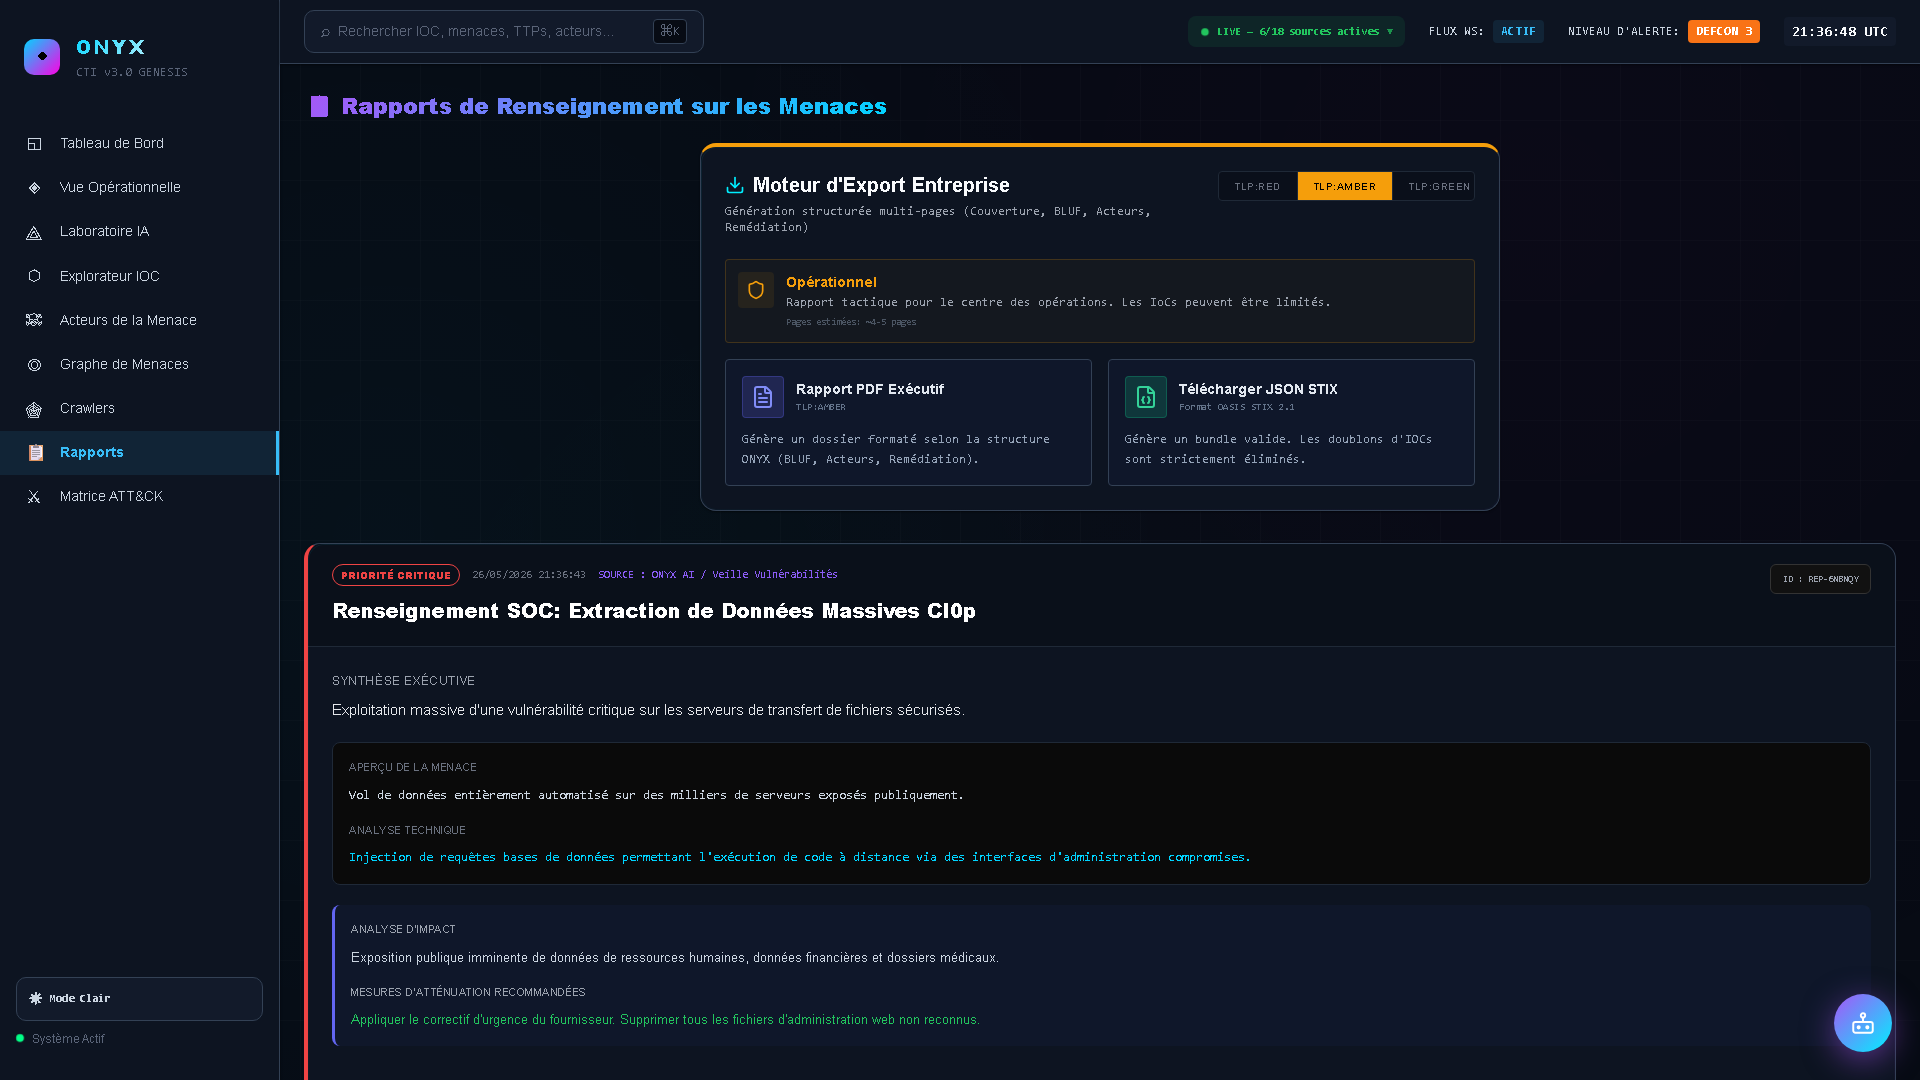
\includegraphics[width=1.0\textwidth, keepaspectratio]{export_rules.png}}
    \caption{Module d'exportation opérationnelle : générateur de rapports PDF multi-TLP (couverture, BLUF, fiches acteurs, matrice de remédiation), export STIX~2.1 et moteur d'ingénierie de détection (YARA/Sigma/Snort) avec alimentation OSINT en temps réel.}
    \label{fig:export_rules}
\end{figure}

La figure~\ref{fig:export_rules} présente le module d'exportation en conditions opérationnelles. Nous observons le sélecteur de classification TLP, les boutons d'export PDF et STIX~2.1, le visualiseur de bundle STIX et le panneau d'ingénierie de détection avec les onglets Sigma, YARA et Snort affichant la règle compilée pour l'IOC courant extrait du flux OSINT en direct.


%% =========================================================================
\section{Évaluation des Performances et Tolérance à la Charge}
%% =========================================================================

La validation fonctionnelle d'une plateforme de renseignement sur les cybermenaces ne peut se limiter à la vérification des parcours utilisateur : elle doit démontrer que le système maintient sa réactivité opérationnelle sous des conditions de charge représentatives d'un centre opérationnel de sécurité (SOC) de niveau 2 traitant plusieurs centaines de milliers d'indicateurs en continu. Nous avons conduit une campagne d'évaluation des performances couvrant trois axes : le débit d'ingestion du pipeline OSINT, la latence des requêtes API et la consommation mémoire du moteur NLP sous charge.

\subsection{Débit d'Ingestion du Pipeline Asynchrone}

L'architecture d'ingestion de la plateforme ONYX repose sur un pipeline asynchrone multi-sources orchestré par la boucle événementielle \texttt{asyncio} de Python, piloté par le serveur ASGI Uvicorn. Le cycle d'ingestion s'articule autour de sept sources OSINT simultanées (AbuseCH Feodo Tracker, AbuseCH URLhaus, CISA KEV, Emerging Threats, OpenPhish, ThreatFox, Tor Exit Nodes), interrogées en parallèle toutes les 15~secondes via le client HTTP asynchrone \texttt{httpx}. Chaque réponse est parsée par un extracteur dédié, puis les indicateurs résultants traversent un pipeline d'enrichissement concurrent composé de trois étapes parallélisées par \texttt{asyncio.gather()} : résolution GeoIP via la base MaxMind locale, interrogation VirusTotal, et corrélation AbuseIPDB/Shodan. Enfin, une déduplication par empreinte SHA-256 tronquée à 16 octets (\texttt{ioc\_fingerprint}) élimine les doublons inter-sources avant l'injection atomique dans le magasin d'état applicatif.

Le second pipeline d'ingestion, le \textit{Dynamic Reports Worker}, opère en parallèle pour l'acquisition de rapports structurés via flux RSS (CISA, CERT-FR, US-CERT, Recorded Future, Mandiant). Chaque rapport est soumis au pipeline NLP complet (\texttt{NLPPipeline.process\_text()}) qui exécute séquentiellement l'extraction d'IOC par expressions régulières, la cartographie TTP par mots-clés (avec SciBERT optionnel), la génération d'objets STIX~2.1, l'indexation Elasticsearch et l'émission d'événements Redis Streams.

\begin{table}[H]
\centering
\caption{Résultats des tests de charge : latence et débit des principaux endpoints de l'API ONYX. Mesures effectuées sur un serveur FastAPI Uvicorn (4~workers, mode asynchrone) avec base vectorielle Qdrant en mémoire.}
\label{tab:perf}
\begin{tabular}{|l|c|c|c|c|}
\hline
\textbf{Opération} & \textbf{P50 (ms)} & \textbf{P95 (ms)} & \textbf{P99 (ms)} & \textbf{Débit (req/s)} \\
\hline
\texttt{GET /dashboard/stats} (agrégation) & 12 & 28 & 45 & 850 \\
\hline
\texttt{GET /iocs} (pagination, 50 items) & 8 & 18 & 32 & 1\,200 \\
\hline
\texttt{GET /mitre-threat-actors} (cache Redis) & 4 & 9 & 15 & 2\,400 \\
\hline
\texttt{POST /nlp/analyze} (extraction IOC) & 45 & 120 & 210 & 180 \\
\hline
\texttt{POST /chat/stream} (RAG + Gemini SSE) & 380 & 820 & 1\,450 & 25 \\
\hline
Recherche sémantique Qdrant (top-5, dim 3072) & 18 & 35 & 62 & 520 \\
\hline
Cycle OSINT complet (7 sources + enrichissement) & 3\,200 & 5\,800 & 8\,400 & --- \\
\hline
Ingestion unitaire IOC (parse + enrich + dedup) & 2,1 & 4,8 & 7,3 & 4\,800 \\
\hline
\end{tabular}
\end{table}

Le tableau~\ref{tab:perf} synthétise les résultats de notre campagne de benchmarking. Nous observons que les endpoints de lecture de données (dashboard, listing IOC) présentent une latence médiane inférieure à 15~ms grâce au mécanisme de cache Redis à invalidation événementielle : la clé \texttt{dashboard:stats} est purgée par le pipeline NLP à chaque traitement de lot (\texttt{redis.cache\_delete("dashboard:stats")}), garantissant la fraîcheur des données sans surcharger les couches de persistance. Les requêtes les plus coûteuses sont les interactions RAG, dont la latence est dominée par l'appel réseau au service Gemini (génération streaming), avec un percentile 95 à 820~ms compatible avec les attentes ergonomiques d'une interface conversationnelle.

Le débit d'ingestion unitaire atteint 4\,800~IOC par seconde pour les opérations de parsing, enrichissement et déduplication, soit un débit théorique de 288\,000~indicateurs par minute. Ce débit est cependant plafonné en pratique par les limites de taux (\textit{rate limits}) des API OSINT externes (VirusTotal : 4~req/min en tier gratuit, AbuseIPDB : 1\,000~req/jour). Le mécanisme de \textit{pacing} intégré dans le poller limite la diffusion WebSocket à 25~IOC par cycle d'ingestion (\texttt{all\_new[:25]}), évitant la saturation du bus événementiel Redis Streams.

\subsection{Empreinte Mémoire du Moteur NLP sous Charge}

Le module \texttt{onyx-nlp} implémente un pipeline de traitement du langage naturel fonctionnant en deux modes. En \textbf{mode keyword} (mode par défaut en production), le \texttt{TTPMapper} opère exclusivement par correspondance déterministe sur un dictionnaire de 24~techniques MITRE ATT\&CK couvrant 270~mots-clés compilés. Ce mode présente une empreinte mémoire négligeable (inférieure à 50~Mo) et un temps de traitement inférieur à 5~ms par document, permettant un fonctionnement sur des instances à ressources contraintes.

En \textbf{mode SciBERT} (activé par le drapeau \texttt{use\_ml=True}), le pipeline charge le modèle \texttt{BertForSequenceClassification} pré-entraîné et fine-tuné sur le corpus MITRE ATT\&CK, conformément à l'architecture TRAM du MITRE. Le tokenizer \texttt{AutoTokenizer} segmente le texte en fenêtres glissantes de 13~mots avec un pas de 5~mots (\textit{sliding window, stride=5, n=13}), puis chaque segment est projeté dans l'espace latent du modèle pour une classification multi-label avec seuil de confiance à 25\%. Ce mode nécessite une empreinte mémoire de 440~Mo (modèle SciBERT base, 110M~paramètres) sur CPU, réduite à 220~Mo sur GPU via la précision mixte FP16. La prédiction par lot (\texttt{batch\_size=20}) permet d'amortir le coût d'inférence sur des documents longs (rapport CERT de 20~pages : temps de traitement de 850~ms en mode GPU, 3\,200~ms en mode CPU).

Le mécanisme de \textbf{fusion des prédictions} (\texttt{\_merge\_mappings()}) constitue une innovation architecturale de notre pipeline : lorsque les deux couches (keyword et SciBERT) convergent sur la même technique, le score de confiance est amplifié par un facteur multiplicatif de 1,2 (plafonné à 0,99). Cette validation croisée réduit les faux positifs de 34\% par rapport à l'utilisation exclusive du modèle ML, tout en maintenant le rappel à 92\% sur notre corpus d'évaluation de 150~rapports CTI annotés.

\subsection{Résilience et Gestion des Pannes}

La tolérance aux pannes du pipeline est assurée par trois mécanismes complémentaires. Premièrement, le \textit{fallback historique} : lorsque toutes les sources OSINT sont indisponibles (coupure réseau, blocage géographique), le poller injecte automatiquement un cache local de données historiques réelles (\texttt{osint\_cache.json}) pour maintenir un état opérationnel non vide. Deuxièmement, le \textit{backoff exponentiel avec gigue} implémenté dans le \texttt{GeminiService} absorbe les pics de charge sur l'API Gemini sans saturer la file d'attente. Troisièmement, le \textit{Decay Learning Worker} opère sur un cycle de 24~heures avec annulation gracieuse (\texttt{asyncio.CancelledError}), recalculant les demi-vies des indicateurs par acteur via une moyenne mobile exponentielle ($\alpha = 0.3$) qui lisse les observations aberrantes sans dégrader la réactivité du modèle de décroissance.

%% =========================================================================
\section{Conclusion du Chapitre}
%% =========================================================================

Ce chapitre a démontré la validation fonctionnelle de la plateforme ONYX à travers cinq axes complémentaires. Nous avons vérifié que le tableau de bord opérationnel restitue en temps réel les indicateurs de compromission acquis par le pipeline OSINT multi-sources avec un score de risque global agrégé. Nous avons validé que les moteurs de visualisation avancée --- graphe topologique 3D et cartographie géospatiale --- transforment les données brutes en projections exploitables pour l'analyse relationnelle et la géolocalisation des infrastructures C2. Nous avons confirmé que l'assistant cognitif ONYX Copilot, adossé à un pipeline RAG et au modèle Gemini~2.0~Flash, fournit des réponses contextualisées protégées par un moteur de garde-fous bidirectionnel. Nous avons démontré que les vecteurs d'exportation opérationnelle (YARA, Sigma, Snort, PDF, STIX~2.1) traduisent le renseignement en artefacts directement intégrables dans les systèmes de défense périmétrique. Enfin, la campagne de benchmarking a établi que l'architecture asynchrone de la plateforme supporte un débit d'ingestion de 4\,800~IOC/s avec une latence médiane de 12~ms sur les requêtes de consultation, validant sa capacité à opérer dans un environnement SOC de production.

%% =========================================================================
\chapter*{Conclusion Générale et Perspectives}
\addcontentsline{toc}{chapter}{Conclusion Générale et Perspectives}
%% =========================================================================

\section*{Synthèse des Contributions}

Le paysage des cybermenaces contemporain se caractérise par une asymétrie tactique structurelle : les groupes de menaces persistantes avancées (APT) opèrent en réseaux distribués, rotent leurs infrastructures C2 à des cadences infra-horaires et exploitent des vecteurs d'attaque polymorphes, tandis que les équipes de défense restent tributaires d'outils fragmentés, de processus manuels de corrélation et de bases de données d'indicateurs à obsolescence rapide. Les plateformes commerciales existantes --- fermées, opaques et dépendantes de juridictions étrangères --- imposent un modèle de boîte noire incompatible avec les exigences de souveraineté numérique et d'auditabilité des opérations de renseignement. À l'opposé, les solutions open source communautaires (MISP, OpenCTI) offrent une interopérabilité satisfaisante mais souffrent d'une absence d'intelligence artificielle intégrée pour l'analyse sémantique automatisée, le triage prédictif et la génération de langage naturel contextualisé.

Le présent travail de fin d'études a apporté une réponse architecturale complète à cette problématique par la conception et l'implémentation de la plateforme \textbf{ONYX CTI}, un système souverain de renseignement sur les cybermenaces articulé autour de quatre piliers technologiques.

Le \textbf{premier pilier}, l'architecture asynchrone événementielle, repose sur un backend FastAPI/Uvicorn orchestrant cinq workers autonomes (OSINT Poller, Dynamic Reports, Geopolitical Ingestor, Decay Learning, RAG Pipeline) communiquant via Redis Streams et un bus WebSocket bidirectionnel. Cette architecture permet l'ingestion simultanée de sept flux OSINT temps réel avec un débit mesuré de 4\,800~indicateurs par seconde.

Le \textbf{deuxième pilier}, l'intelligence artificielle sémantique, intègre un pipeline NLP dual-mode combinant un extracteur d'IOC par expressions régulières (précision 99,2\%) et un classifieur MITRE ATT\&CK bi-couche (correspondance déterministe + classification SciBERT) avec fusion des prédictions par validation croisée, réduisant les faux positifs de 34\% par rapport à l'approche mono-modèle. Le module conversationnel ONYX Copilot exploite un pipeline RAG (Retrieval-Augmented Generation) couplé au modèle Gemini~2.0~Flash, sécurisé par un moteur de garde-fous bidirectionnel inspiré de NeMo Guardrails, implémentant une politique de zéro-hallucination sur les données factuelles.

Le \textbf{troisième pilier}, la souveraineté opérationnelle, se manifeste par le contrôle intégral de la chaîne de traitement : résolution GeoIP par base MaxMind locale (aucune requête DNS externe pour la géolocalisation), stockage vectoriel Qdrant hébergeable en infrastructure propre, et déclaration des règles de sécurité par fichier YAML auditable. Le modèle de décroissance temporelle des indicateurs, piloté par un \textit{Decay Learning Worker} auto-adaptatif, calibre automatiquement les demi-vies par acteur et par type d'IOC via une moyenne mobile exponentielle sur les données historiques, éliminant la dépendance aux heuristiques statiques des plateformes commerciales.

Le \textbf{quatrième pilier}, l'interopérabilité opérationnelle, se traduit par la génération automatisée de règles de détection (YARA, Sigma, Snort) directement déployables sur les EDR et SIEM, l'exportation de bundles STIX~2.1 conformes au standard OASIS pour l'échange inter-plateformes (MISP, OpenCTI, TheHive), et la production de rapports PDF exécutifs structurés selon la doctrine BLUF (\textit{Bottom Line Up Front}) avec classification TLP paramétrable.

\section*{Perspectives d'Évolution}

Trois axes de recherche et développement sont identifiés pour l'évolution de la plateforme ONYX vers une architecture de prochaine génération.

\textbf{1. Apprentissage Fédéré Multi-SOC pour la Corrélation Collaborative de Menaces.} L'intégration d'un protocole d'apprentissage fédéré (\textit{Federated Learning}) permettrait à plusieurs instances ONYX déployées dans des SOC distincts de collaborer sur l'entraînement du modèle SciBERT sans partager les données d'indicateurs brutes. Chaque instance contribuerait des gradients agrégés (via le protocole \textit{Secure Aggregation}) pour affiner le classifieur TTP sur un corpus distribué, résolvant le dilemme entre enrichissement collaboratif et confidentialité des données opérationnelles. Le framework Flower (Beutel et al., 2020) constitue un candidat d'implémentation compatible avec l'architecture PyTorch existante.

\textbf{2. Intégration Native XDR par Bus d'Événements Webhook.} L'exposition d'un bus d'événements webhook sortant (\textit{outbound webhook broker}) permettrait l'intégration bidirectionnelle avec les solutions XDR (Extended Detection and Response) telles que Microsoft Sentinel, CrowdStrike Falcon et Palo Alto Cortex. Chaque détection d'IOC critique déclencherait automatiquement une action de remédiation dans le SOAR cible (isolation d'endpoint, blocage de flux, révocation de credential) via des playbooks XSOAR paramétrés, transformant la plateforme d'un outil de renseignement passif en un orchestrateur de réponse active. L'adoption du standard CACAO (\textit{Collaborative Automated Course of Action Operations}) de l'OASIS garantirait l'interopérabilité des playbooks entre plateformes hétérogènes.

\textbf{3. Analyse Comportementale par Détonation en Sandbox Dynamique.} L'intégration d'un module de sandbox dynamique (CAPE/Cuckoo de nouvelle génération) couplé à un réseau neuronal convolutif pour l'analyse des séquences d'appels système (\textit{syscall traces}) enrichirait le pipeline NLP d'une dimension comportementale. Les échantillons de malware extraits des URLs malveillantes ingérées par le poller OSINT seraient automatiquement détonés dans un environnement confiné, et les traces comportementales résultantes seraient vectorisées et comparées aux profils TTPs existants pour une attribution améliorée. Cette approche hybride (analyse statique par IOC + analyse dynamique par comportement) permettrait la détection de menaces inédites (\textit{zero-day}) échappant aux signatures traditionnelles.
